\documentclass[a4paper, 11pt, titlepage, twoside, openany]{book}
\usepackage{plain}
\usepackage{setspace}
% Layout
\usepackage[
  paperheight=29.7cm,
  paperwidth=21cm,
  outer=1.5cm,
  inner=2.5cm,
  top=2cm,
  bottom=2cm
]{geometry}
% Chapter
\usepackage{titlesec}
\singlespacing
\setcounter{secnumdepth}{3}
\setcounter{tocdepth}{3}
% Letter
\usepackage[utf8]{inputenc}
% Language
\usepackage[english]{babel}
% PDF/A
\usepackage[a-1b]{pdfx}
% Image
\usepackage{graphicx}
\usepackage{wrapfig}
\usepackage{stackengine}
\usepackage{etoolbox}
\BeforeBeginEnvironment{wrapfigure}{\setlength{\intextsep}{0pt}}
% Hyperlink
\usepackage{xurl}
\usepackage[pdfa]{hyperref}
\hypersetup{breaklinks=true}
% List
\usepackage{enumitem}
\usepackage{listings}

\usepackage{xcolor}
\usepackage{hhline}

\lstdefinestyle{Assembly}{ backgroundcolor=
\color{lightgray!20}
, commentstyle=
\color{green}
, keywordstyle=
\color{blue}
, numberstyle=\tiny
\color{gray}
, stringstyle=
\color{red}
, numbers=left, stepnumber=1, numbersep=5pt, frame=single, tabsize=4, captionpos=b,
breaklines=true, breakatwhitespace=false, showspaces=false, showstringspaces=false,
showtabs=false, morekeywords={add, ret, jal, jalr, la, ecall, mv, call, auipc, addi, sw, lw},
xleftmargin=10pt }

\lstdefinestyle{CStyle}{ backgroundcolor=
\color{lightgray!20}
, commentstyle=
\color{green}
, keywordstyle=
\color{blue}
, numberstyle=\tiny
\color{gray}
, stringstyle=
\color{red}
, numbers=left, stepnumber=1, numbersep=5pt, frame=single, tabsize=4, captionpos=b,
breaklines=true, breakatwhitespace=false, showspaces=false, showstringspaces=false,
showtabs=false, xleftmargin=10pt, language=C }

\lstdefinelanguage[RISC-V]{Assembler}{ alsoletter={.}, % allow dots in keywords
alsodigit={0x}, % hex numbers are numbers too!
morekeywords=[1]{ % instructions
lb, lh, lw, lbu, lhu, sb, sh, sw, sll, slli, srl, srli, sra, srai, add, addi, sub, lui, auipc, xor, xori, or, ori, and, andi, slt, slti, sltu, sltiu, beq, bne, blt, bge, bltu, bgeu, j, jr, jal, jalr, ret, scall, break, nop },
morekeywords=[2]{ % sections of our code and other directives
.align, .ascii, .asciiz, .byte, .data, .double, .extern, .float, .globl, .half, .kdata, .ktext, .set, .space, .text, .word },
morekeywords=[3]{ % registers
zero, ra, sp, gp, tp, s0, fp, t0, t1, t2, t3, t4, t5, t6, s1, s2, s3, s4, s5, s6, s7, s8, s9, s10, s11, a0, a1, a2, a3, a4, a5, a6, a7 },
morecomment=[l]{;}, % mark ; as line comment start
morecomment=[l]{\#}, % as well as # (even though it is unconventional)
morestring=[b]", % mark " as string start/end
morestring=[b]' % also mark ' as string start/end
}

\definecolor{mauve}{rgb}{0.58,0,0.82}

\lstset{ basicstyle=\ttfamily, % very small code
breaklines=true, % break long lines
commentstyle=\itshape
\color{green!50!black}
, % comments are green
keywordstyle=[1]
\color{blue!80!black}
, % instructions are blue
keywordstyle=[2]
\color{orange!80!black}
, % sections/other directives are orange
keywordstyle=[3]
\color{red!50!black}
, % registers are red
stringstyle=
\color{mauve}
, % strings are from the telekom
identifierstyle=
\color{teal}
, % user declared addresses are teal
frame=l, % black line on the left side of code
language=[RISC-V]Assembler, % all code is RISC-V
tabsize=4, % indent tabs with 4 spaces
showstringspaces=false % do not replace spaces with weird underlines
}

% Document
\begin{document}
  % Cover
  \pagenumbering{gobble}
  \pagestyle{plain}
\thispagestyle{empty}

\begin{center}
  \begin{figure}[h!]
    \centering
    
\includegraphics[width=.6\textwidth]{images/logo/unitn.png}
  \end{figure}

  \vspace{2 cm}
  \LARGE{Department of Information Engineering and Computer Science\\}

  \vspace{1 cm}
  \Large{Master's Degree in\\ Computer Science}

  \vspace{2 cm}
  \Large\textsc{Final Dissertation\\}
  \vspace{1 cm}
  \Huge\textsc{Design and implementation of trusted services on RISC -V: the
  case of Control Flow Integrity\\}
  \vspace{0.5 em}
  \Large{\textit{A lightweight Control Flow Integrity Enforcer for embedded RISC-V systems}}

  \vspace{2 cm}
  \begin{tabular*}{\textwidth}{c @{\extracolsep{\fill}} c}
    \Large{Supervisor}      & \Large{Student}        \\
    \Large{Bruno Crispo}    & \Large{Davide Moletta} \\
    \Large{Co-Supervisor}   & \Large{239272}         \\
    \Large{Michele Grisafi} & {}                     \\
  \end{tabular*}

  \vspace{2 cm}
  \Large{Academic year 2023/2024}
\end{center}
  \clearpage

  % Acknowledgements
  %\thispagestyle{empty}

\begin{center}
  {\bf \Huge Acknowledgements}
\end{center}

\vspace{4cm}
\emph{Thanks to ...}
  \clearpage
  \pagestyle{plain}

  % Table of Contents
  \frontmatter
  \pagenumbering{Roman}
  \tableofcontents
  \clearpage
  \begingroup
  \pagestyle{empty}
  \cleardoublepage
  \endgroup

  % Start page numbering
  \mainmatter

  % Group to define space between chapters
  \begingroup
  % Override format of title chapter
  \titleformat{\chapter} {\normalfont\Huge\bfseries}{\thechapter}{1em}{} \titlespacing*{\chapter}{0pt}{0.59in}{0.02in}
  \titlespacing*{\section}{0pt}{0.20in}{0.02in} \titlespacing*{\subsection}{0pt}{0.10in}{0.02in}
  \titlespacing*{\subsubsection}{0pt}{0.05in}{0.02in}

  % Abstract
  \chapter*{Abstract}
\label{cha:abtract}
\addcontentsline{toc}{chapter}{Abstract}

\lipsum[1]

  % Chapters
  \chapter{Introduction}
\label{cha:introduction}

This chapter serves as an introduction to this thesis, where we present a new security
infrastructure for \textit{RISC-V}-based embedded devices. The proposed solution
aims to provide security features to mitigate control flow hijacking attacks and
allow the execution of untrusted user code. This result is accomplished by
enforcing Control Flow Integrity on the target code. Moreover, great focus has
been put on providing an efficient and lightweight infrastructure that complies
with the limited hardware capabilities of embedded devices.

\section{Problem}
\label{sec:intro_context}

Embedded devices are now an integral part of daily life, powering a wide range
of applications that span from smart home assistants and appliances to connected
furniture. These compact computing units have expanded across numerous domains,
supporting diverse tasks that enhance convenience, efficiency, and connectivity
in everyday environments. A defining feature of embedded devices is their network
connectivity, which links them to the broader Internet of Things (IoT) ecosystem.
According to the ``\textit{State of IoT Summer 2024}'' report, $16.6$ billion devices
were connected by the end of $2023$, a figure expected to rise to $18.8$ billion
during $2024$\footnote{\url{https://iot-analytics.com/number-connected-iot-devices/}}.
These devices perform critical functions across industries ranging from consumer
electronics to industrial automation and healthcare. However, they are often
resource-constrained and designed to perform specific tasks with minimal power
and computational resources, making them inherently vulnerable to cyber threats.
In $2022$, approximately $112$ million IoT cyberattacks were reported globally\footnote{\url{https://1nce.com/en-us/resources/news/blog/iot-cybersecurity-landscape}},
and this figure continues to escalate, with the first half of $2024$ witnessing
a $107\%$ increase in attacks as highlighted by \textit{SonicWall}'s ``\textit{2024
Mid-Year Cyber Threat Report}''\footnote{\url{https://www.sonicwall.com/threat-report}}.
Consequently, embedded device security is an increasingly pressing concern, as
attacks on these devices can result in data breaches, unauthorized system control,
or disruptions to essential services.

Among the potential threats, we have Software-based, Network-based, and Side-based
attacks that an attacker may use to impact the Confidentiality, Integrity, and Availability
of a system. One notable example of a Network-based attack is the \textit{Man-In-The-Middle}
(MITM) attack. In this scenario, a malicious actor intercepts the communication between
two parties, thereby gaining unauthorized access to sensitive data such as
cryptographic keys, login credentials, and personal information. This breach can
lead to severe consequences, including data theft, identity fraud, and loss of
trust in communication channels. Another example is the threat posed by control flow
hijacking attacks, a family of cyber attacks that aim at disrupting the normal
execution flow of a program to execute arbitrary code or gain control of the
target device. These types of attacks may result in additional threats, for
example, if an attacker manages to gain control of a significant number of devices,
they can form what is known as a \textit{Botnet}. This network of infected
devices can be orchestrated to launch large-scale \textit{Distributed Denial of
Service} (DDoS) attacks against external systems. In a DDoS attack, the botnet floods
a targeted server or network with excessive traffic, overwhelming it and
rendering it unable to process legitimate requests. This disruption can lead to service
outages, financial losses, and damage to the organization's reputation.

With all this information it is easy to understand why embedded devices have become
a suitable target for cyber attacks and why this is a major security concern. It
would be relatively ``easy'' to think of implementing state-of-the-art security
solutions to protect these devices, however, the problem is that many of them
have limited hardware resources as they may be designed to carry out simple
tasks. This means we must apply security measures within the device's capabilities
without affecting its performance. This is indeed a challenge because, in embedded
systems security, we often need to design tailored security features to protect
the device while maintaining efficiency high. Here, we discuss how we aim to
contribute to the world of embedded security with the presented project.

\section{Goals}
\label{sec:intro_goals}

This project introduces innovative security features designed specifically for embedded
\textit{RISC-V}-based systems. The primary objective of this project is to establish
a robust software-based Control Flow Integrity enforcer that allows secure execution
of untrusted user code. This is particularly crucial in scenarios where running
potentially malicious or unverified code can pose significant risks to system
integrity and security. A key focus of the project is to ensure that Control Flow
Integrity remains intact throughout the execution process, thereby preventing
any unauthorized modifications to the flow of control within the program. This protection
is achieved by enforcing backward and forward edge protection using state-of-the-art
techniques such as a shadow stack and Control Flow Graph validation. Moreover, Physical
Memory Protection is integrated into the project to protect critical memory areas.

Additionally, considering that this project aims at protecting embedded devices,
which often have constrained hardware resources, special emphasis has been
placed on employing optimization techniques. These techniques are designed to minimize
the impact of the Control Flow Integrity enforcer on both memory consumption and
execution performance. We aim to enable the secure execution of untrusted code
without imposing excessive overhead that could hinder the functionality of
resource-limited embedded systems.

Furthermore, throughout the development process, we have adhered to the open and
modular design principles inspired by \textit{RISC-V}. This commitment to
modularity and openness has resulted in a highly adaptable infrastructure that
can be easily modified to suit a variety of deployment scenarios. With this, we
aim to streamline the deployment process, making it faster and more efficient in
diverse environments, thereby enhancing the overall utility and effectiveness of
provided security features.

By integrating Control Flow Integrity mechanisms, this project aims to enhance the
security of control paths within \textit{RISC-V} systems. Control Flow Integrity
ensures that the execution of the embedded system remains trusted and reliable,
safeguarding it from potential exploits or vulnerabilities that could compromise
its operations. Through this advancement, the project not only improves the
robustness of the \textit{RISC-V} instruction set architecture but also contributes
to the overall resilience of embedded applications in various critical fields.

\section{Structure}
\label{sec:intro_structure}

Following this introduction, chapter \ref{cha:background} presents a comprehensive
background about the problem, security techniques, and related works that provide
a similar solution to the one presented in this thesis. We start by describing
the problem, its severity, and the relevant attacks we aim to mitigate. Secondly,
we discuss state-of-the-art security measures that aim at mitigating control
flow hijacking attacks, strongly focusing on Control Flow Integrity. Lastly, we present
related projects discussing what differentiates them from our approach.

In chapter \ref{cha:threatmodel} we provide the threat model and assumptions for
this project. We state the problem and the target of our security measures. Also,
we discuss assumptions we made about the threat scenario and the capabilities of
the attacker.

Chapter \ref{cha:riscv} presents the foundational concepts of the \textit{RISC-V}
Instruction Set Architecture. In this chapter, we focus only on essential information
needed for a complete understanding of the architectural basis of the project.

Chapter \ref{cha:project} details the implementation specifics of the Control Flow
Integrity enforcer, discussing critical features such as forward and backward
edge control mechanisms and the use of Physical Memory Protection to create
secure memory spaces. To validate the effectiveness of the project in real-world
scenarios, this chapter also introduces a Proof of Concept which will exemplify
how the project addresses critical security threats, illustrating its impact on device
resilience and system integrity.

A subsequent security analysis, discussed in chapter \ref{cha:ta}, will describe
the testing methodologies used to assess the project's effectiveness in identifying
and preventing control flow hijacking attacks. Moreover, we discuss the security
limitations of the Control Flow Integrity enforcer identifying any potential vulnerabilities
that may need further consideration.

A performance analysis is also provided in chapter \ref{cha:pa}, where the trade-offs
between security and system efficiency are evaluated. This analysis will help highlight
the strengths and limitations of the project and explain why it represents a feasible
solution for enhancing the security of \textit{RISC-V}-based embedded devices. During
this chapter we showcase test results for time and memory consumption,
showcasing the average overhead of the project. Lastly, we provide insights on
optimization ideas to further increase performance.

Additionally, the thesis explores the potential integration of a Real-Time Operating
System (RTOS) for embedded devices during chapter \ref{cha:rtos}. In particular,
we propose the integration of \textit{FreeRTOS} and \textit{Zephyr RTOS}, two
widely-used Real-Time Operating Systems. This integration could extend the project's
applicability, enabling more complex programs to operate under the Control Flow
Integrity enforcer. By supporting an established RTOS like \textit{FreeRTOS}, the
project could broaden its reach and utility, making it suitable for a larger
variety of use cases in the embedded device domain.

Finally, in chapter \ref{cha:future}, we discuss future enhancements we plan to
integrate. In this chapter, we mainly focus on security and performance-oriented
solutions that could broaden the security of the project while reducing its
impact on the device's performance.

In summary, this thesis presents a novel approach to securing \textit{RISC-V}
microcontrollers, leveraging Control Flow Integrity to protect against control flow
hijacking attacks and providing a secure foundation for running potentially unsafe
code. Through detailed technical exploration, demonstration, and analysis, this work
aims to contribute a significant advancement to the field of embedded device security,
addressing both current and emerging threats in the IoT landscape.
  \chapter{RISC-V}
\label{cha:riscv}

\textit{RISC-V} is an open standard Instruction Set Architecture (ISA) based on the
principles of Reduced Instruction Set Computing (RISC). Unlike proprietary ISAs
like \textit{x86} and \textit{ARM}, \textit{RISC-V} is designed to be open and
free, enabling anyone to develop compatible hardware and software without licensing
fees. This openness makes it highly appealing for academia, research, and
commercial applications, as companies can design custom processors tailored to specific
applications while avoiding vendor lock-in.

The \textit{RISC-V} ISA has been defined as an interface to a wide variety of
implementations rather than as the design of a particular hardware. This means that
the same ISA can be used with many processors and is not tailored to a specific one
leaving space for customization, flexibility, and reusability.

In the following sections, we provide a detailed background on the \textit{RISC-V}
ISA and the aspects that are necessary to understand the underlying infrastructure
of the project\footnote{Every information will refer to the $32$-bit \textit{RV32I}
ISA since it is the one utilized in the project.}\footnote{Most of the
information in this chapter is taken from both the Unprivileged and Privileged
Specifications\cite{specifications} published from \textit{RISC-V} International.}.

\section{RISC-V ISA Overview}
\label{sec:riscv_isa}

The \textit{RISC-V} ISA is structured around a minimal base integer ISA, which
is mandatory for all implementations. Even if we refer to the ``base integer ISA''
there are actually four base ISAs within the \textit{RISC-V} family: \textit{RV32I},
\textit{RV64I}, \textit{RV32E}, and \textit{RV64E}, each differing primarily in the
width of integer registers ($32$ or $64$ bits) and the number of available registers
(\textit{E} ISAa support half the number of registers). These variations support
different use cases, from small microcontrollers (\textit{RV32E} and \textit{RV64E})
to larger systems (\textit{RV64I}). Moreover, RISC-V International is currently working
on a $128$-bit ISA known as \textit{RV128I}.

These base ISAs are designed to provide the bare minimum instructions for
essential software tools while allowing for extensive customization and
specialization through additional extensions.

To accommodate customization, \textit{RISC-V} divides each instruction-set
encoding space into three categories:
\begin{itemize}[noitemsep]
  \item Standard extensions and encodings are defined by \textit{RISC-V
    International}. Such extensions are designed to not conflict with each other;

  \item Reserved encodings are currently not defined and are saved for future use;

  \item Custom encodings are made available for vendor-specific non-standard extensions.
\end{itemize}
This segmentation supports the creation of specialized ISAs without conflicting with
the core architecture.

\section{RISC-V Extensions}
\label{sec:riscv_extensions}

\textit{RISC-V}'s standard extensions are officially supported and maintained by
\textit{RISC-V International}. They add functionality to the base ISA while ensuring
compatibility across different implementations. These extensions are designed to
enhance performance, reduce power consumption, or expand the processor's
capability to handle specific tasks efficiently (standard extensions can be seen
in Table \ref{tab:extensions}).

Standard extensions can be used together to obtain the needed capabilities for
each specific situation. Moreover, \textit{RISC-V}'s open architecture allows for
the creation of custom extensions, enabling developers to implement specialized
instructions for domain-specific optimizations. However, while these custom
extensions provide powerful optimizations, they are not standardized, so
compatibility across different implementations is not guaranteed.

The ISA used in this project is \textit{RV32IMC\_ZICSR} where \textit{RV32I}
stands for the base integer ISA, \textit{M} is used to provide multiplication
and division instructions, and \textit{C} is used to provide compressed
instructions which are useful in restricted environments like embedded devices. \textit{ZICSR}
is an additional extension that will be discussed later.

\begin{table}
  \centering
  \begin{tabular}{|c|c|}
    \hline
    \textbf{Extension Code} & \textbf{Description}                \\
    \hhline{==} A           & Atomic instructions                 \\
    \hline
    B                       & Bit manipulation                    \\
    \hline
    C                       & Compressed instructions             \\
    \hline
    D                       & Double-precision floating-point     \\
    \hline
    F                       & Single-precision floating-point     \\
    \hline
    G                       & Shorthand for IMAFD extensions      \\
    \hline
    H                       & Hypervisor extension                \\
    \hline
    J                       & Dynamically translated languages    \\
    \hline
    L                       & Decimal floating-point              \\
    \hline
    M                       & Integer multiplication and division \\
    \hline
    N                       & User-level interrupts               \\
    \hline
    P                       & Packed-SIMD instructions            \\
    \hline
    Q                       & Quad-precision floating-point       \\
    \hline
    S                       & Supervisor mode                     \\
    \hline
    T                       & Transactional memory                \\
    \hline
    V                       & Vector operations                   \\
    \hline
  \end{tabular}
  \caption{\textit{RISC-V} Standard Extensions}
  \label{tab:extensions}
\end{table}

\section{RISC-V Base Instruction Formats}
\label{sec:riscv_bif}

The base \textit{RISC-V} ISA has fixed-length $32$-bit instructions that must be
aligned to a four-byte boundary in memory. However, the \textit{C} extension for
compressed instructions relaxes this requirement and allows to inclusion of $16$-bit
long instructions aligned at a two-byte boundary.

The base \textit{RV32I} ISA uses four main instruction formats: \textit{R},
\textit{I}, \textit{S}, and \textit{U}, all fixed at $32$ bits in length (shown in
Figure \ref{fig:instrformats}).

Additionally, RV32I includes formats \texttt{B} and \texttt{J} (shown in Figure
\ref{fig:extrainstrformats}), which vary in immediate encoding to optimize
hardware design. The immediate structure across formats is designed to minimize hardware
complexity and overlap, focusing on efficiency for both compilation and runtime
execution. Sign-extension and fixed bit positioning help reduce hardware costs and
reduce complexity in simple implementations.

\begin{figure}[htbp]
  \centering
  \def\stackalignment{r}\stackunder{ 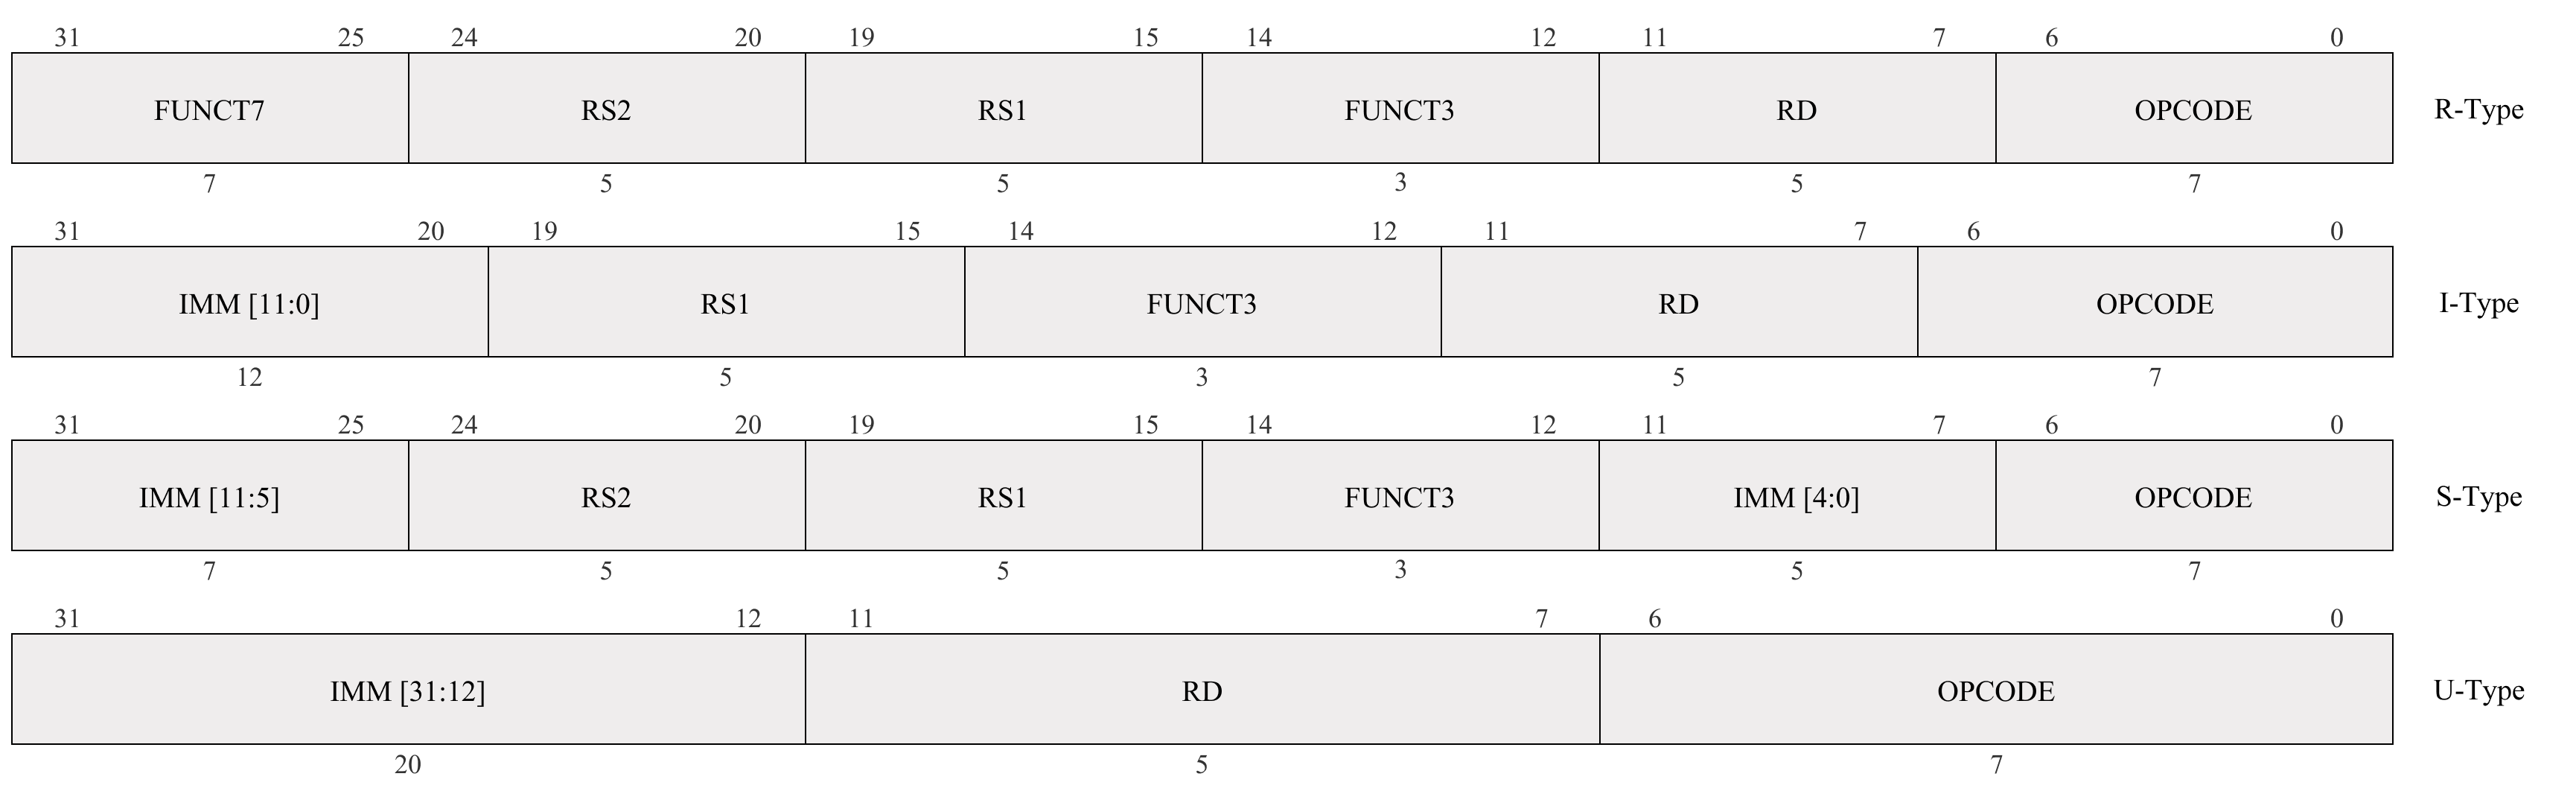
\includegraphics[width=.9\linewidth]{images/instrformats.png}}
  {\scriptsize Source: \href{https://drive.google.com/file/d/1uviu1nH-tScFfgrovvFCrj7Omv8tFtkp/view}{\textit{RISC-V} Unprivileged Manual, page $23$}}
  \caption{RISC-V Base Instruction Formats}
  \label{fig:instrformats}
\end{figure}

\begin{figure}[htbp]
  \centering
  \def\stackalignment{r}\stackunder{ 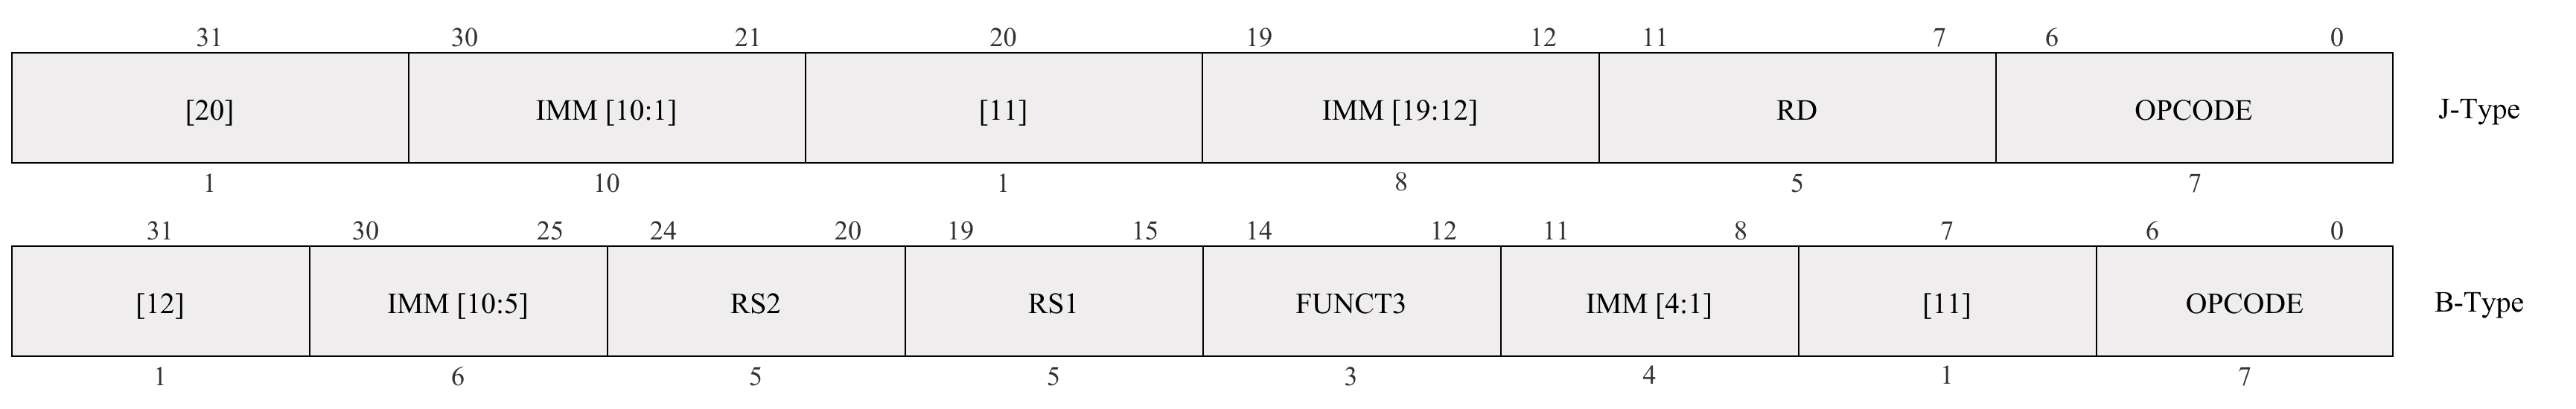
\includegraphics[width=.9\linewidth]{images/extrainstrformats.png} } %
  {\scriptsize Source: \href{https://drive.google.com/file/d/1uviu1nH-tScFfgrovvFCrj7Omv8tFtkp/view}{\textit{RISC-V} Unprivileged Manual, page $24$}}
  \caption{RISC-V Extra Instruction Formats}
  \label{fig:extrainstrformats}
\end{figure}

The \textit{RISC-V} ISA keeps the source (\textit{RS1} and \textit{RS2}) and
destination (\textit{RD}) registers in the same position to simplify instruction
decoding. Immediate values (\textit{IMM}) are always sign-extended and generally
stored in the most significant available bits. Lastly, \textit{FUNCT3}, \textit{FUNCT7}
and \textit{OPCODE} are used to define the operation.

\subsection{Control Transfer Instructions}
\label{subsec:riscv_controltransfer}

In this subsection, we explain \textit{RISC-V}'s control transfer instructions
which are fundamental for this project.

\textit{RV32I} defines two types of control transfer instructions: unconditional
jumps and conditional branches.

\subsubsection{Unconditional Jumps}
\label{subsubsec:riscv_unconditionalj}

\textit{RISC-V} defines two types of unconditional jumps: jump and link (\textit{JAL})
and jump and link register (\textit{JALR}).

The \textit{JAL} instruction is encoded using the \textit{J}-type format. The
immediate offset is sign-extended and added to the address of the jump
instruction (current \textit{pc}\footnote{\textit{pc} stands for program counter
and holds the address of the current instruction}) to determine the jump target
address. As a result, jumps can target a range within $\pm 1 MiB$ from their
address. Moreover, \textit{JAL} stores the address of the instruction following the
jump ($\textit{pc}+ 4$) into the destination register \textit{RD}.

The \textit{JALR} instruction is encoded using the \textit{I}-type format. The immediate
offset is sign-extended and added to the source register \textit{RS1} to
determine the jump target address (also the least-significant bit of the result is
set to $0$). Similarly to \textit{JAL}, \textit{JALR} stores the address of the
instruction following the jump ($\textit{pc}+ 4$) into the destination register
\textit{RD}.

Lastly, a plain unconditional jump is provided under the pseudo-instruction
\textit{J} and it is simply encoded as a \textit{JAL} instruction with
$\textit{RD}= x0$.

\subsubsection{Conditional Branches}
\label{subsubsec:riscv_conditionalb}

\textit{RISC-V} defines six branch instructions that compare two registers. \textit{BEQ}
and \textit{BNE} take the branch if registers \textit{RS1} and \textit{RS2} are equal
or different respectively. \textit{BLT} and \textit{BLTU} take the branch if
\textit{RS1} is less than \textit{RS2}, using signed and unsigned comparison respectively.
Lastly, \textit{BGE} and \textit{BGEU} take the branch if \textit{RS1} is
greater than or equal to \textit{RS2}, using signed and unsigned comparisons
respectively.

All conditional branch instructions are encoded using the \textit{B}-type format.
The immediate offset is sign-extended and added to the address of the branch
instruction (current \textit{pc}) to determine the branch target address. As a
result, conditional branches can target a range within $\pm 4 \textit{KiB}$ from
their address.

\subsection{Environment Calls and Breakpoints}
\label{subsec:riscv_ecalls}

\textit{RISC-V} defines two classes of \textit{SYSTEM} instructions which are
used to access system functionalities that may require privileged access. These instructions
are encoded using the \textit{I}-type format. The two classes are those that read-modify-write
Control and Status Registers, and all other potentially privileged instructions.

Control and Status Registers will be discussed later, while among the second class
of \textit{SYSTEM} instructions, we need to define \textit{ECALL} and \textit{EBREAK}.
\textit{ECALL} is used to perform a service request to the execution environment.
The Execution Environment Interface (EII) defines how parameters should be
passed. Instead, \textit{EBREAK} is used to return control to a debugging environment.

\section{RISC-V Exceptions, Traps and Interrupts}
\label{sec:riscv_eti}

In \textit{RISC-V}, exceptions are unusual conditions tied to the execution of
an instruction within the \textit{hart}\footnote{A \textit{hart} in \textit{RISC-V}
is defined as a hardware thread}, while interrupts are external asynchronous events
that may cause an unexpected control transfer within the \textit{hart}. Both exceptions
and interrupts lead to a trap, which causes a control transfer to a trap handler.

Traps in RISC-V can have four possible effects, each corresponding to how the trap
is managed:

\begin{itemize}
  \item Contained Trap: The trap is visible to software in the current execution
    environment and is handled within it. For example, in an EII that provides
    both Machine and User mode , an \textit{ECALL} made by user-mode will generally
    result in a transfer of control to a machine-mode handler within the same \textit{hart};

  \item Requested Trap: A synchronous exception explicitly requesting the
    execution environment to perform an action on behalf of the software inside
    the environment. The software may or may not resume execution on the \textit{hart}
    afterward;

  \item Invisible Trap: The execution environment handles the trap transparently,
    so the running software is unaware of it. An example is handling device
    interrupts for a different job. In this case, the software is not aware of
    the trap and the execution continues normally;

  \item Fatal Trap: This indicates a critical failure, causing the execution environment
    to terminate execution. An example is failing a virtual-memory page-protection
    check.
\end{itemize}

\begin{table}
  \centering
  \begin{tabular}{|c|c|c|c|c|}
    \hline
    \textbf{}                           & \textbf{Contained} & \textbf{Requested} & \textbf{Invisible} & \textbf{Fatal} \\
    \hhline{=====} Execution terminates & No                 & No                 & No                 & Yes            \\
    \hline
    Software is oblivious               & No                 & No                 & Yes                & Yes            \\
    \hline
    Handled by environment              & No                 & Yes                & Yes                & Yes            \\
    \hline
  \end{tabular}
  \caption{RISC-V privilege levels}
  \label{tab:traps}
\end{table}

As we will see later, traps are handled thanks to a trap vector table which is
responsible for managing the trap, deciding the outcome, and resuming the
execution when needed.

\section{RISC-V Privilege Levels}
\label{sec:riscv_privileges}

\textit{RISC-V} defines multiple privilege levels to manage access to system
resources and control execution modes. These privilege levels are designed to provide
a secure and efficient framework for managing different software components,
such as operating systems, hypervisors, and user applications.

As it's possible to see in Table \ref{tab:priv} \textit{RISC-V} implements three
different privilege levels with the following characteristics:

\begin{itemize}
  \item Machine Mode (M-mode): Machine mode is the most privileged and
    fundamental level in the \textit{RISC-V} architecture. It is the only
    required privilege level in all \textit{RISC-V} implementations and provides
    complete access to hardware resources and system configurations. It is
    responsible for configuring the hardware, setting up system resources, and
    initializing other privilege levels. Furthermore, trap handling is performed
    by M-mode;

  \item Supervisor Mode (S-mode): Supervisor mode is an optional privilege level
    designed for running operating systems or hypervisors. It offers more privileges
    than U-mode but less than M-mode. S-mode enables an operating system to
    manage resources and control hardware with enough authority while ensuring
    that user applications cannot access or alter critical system configurations;

  \item User Mode (U-mode): User mode is the least privileged level and is
    designed for running user-level applications. It restricts access to critical
    system resources, ensuring that any malicious or faulty application cannot
    compromise the overall system. U-mode's restricted environment makes it ideal
    for running user applications securely, providing a balance between
    performance and protection.
\end{itemize}

\begin{table}
  \centering
  \begin{tabular}{|c|c|c|c|}
    \hline
    \textbf{Level}  & \textbf{Encoding} & \textbf{Name}    & \textbf{Abbreviation} \\
    \hhline{====} 0 & 00                & User/Application & U                     \\
    \hline
    1               & 01                & Supervisor       & S                     \\
    \hline
    2               & 10                & Reserved         & -                     \\
    \hline
    3               & 11                & Machine          & M                     \\
    \hline
  \end{tabular}
  \caption{RISC-V privilege levels}
  \label{tab:priv}
\end{table}

\section{RISC-V General Purpose Registers}
\label{sec:riscv_reg}

The base \textit{RISC-V} ISA provides $32$ general purpose registers all $32$ bits
wide. Table \ref{tab:registers} depicts all the described registers.

Except for \textit{x0} which is hardwired to $0$ no other registers are assigned
to a specific role. However, the standard calling convention uses:
\begin{itemize}
  \item register \textit{x1}: as return address for a \textit{JAL} or \textit{JALR}
    instruction;

  \item register \textit{x5}: as an alternate link register for \textit{JAL} and
    \textit{JALR} instructions;

  \item register \textit{x2}: as the stack pointer;

  \item \textit{t}-registers: as temporary registers which are to be saved by the
    caller when needed;

  \item \textit{a}-registers: as function arguments and return values;

  \item \textit{s}-registers: as saved registers which are to be saved by the callee
    when needed.
\end{itemize}

\begin{table}
  \centering
  \begin{tabular}{|c|c|c|}
    \hline
    \textbf{Register}        & \textbf{Alias}  & \textbf{Calling Convention Description}    \\
    \hhline{===} \textit{x0} & \textit{zero}   & Hard-wired zero                            \\
    \hline
    \textit{x1}              & \textit{ra}     & Return address                             \\
    \hline
    \textit{x2}              & \textit{sp}     & Stack pointer                              \\
    \hline
    \textit{x3}              & \textit{gp}     & Global pointer                             \\
    \hline
    \textit{x4}              & \textit{tp}     & Thread pointer                             \\
    \hline
    \textit{x5}              & \textit{t0}     & Temporary register/alternate link register \\
    \hline
    \textit{x6-x7}           & \textit{t1-t2}  & Temporary registers                        \\
    \hline
    \textit{x8}              & \textit{s0/fp}  & Saved register/frame pointer               \\
    \hline
    \textit{x9}              & \textit{s1}     & Saved register                             \\
    \hline
    \textit{x10-x11}         & \textit{a0-a1}  & Function arguments/return values           \\
    \hline
    \textit{x12-x17}         & \textit{a2-a7}  & Function arguments                         \\
    \hline
    \textit{x18-x27}         & \textit{s2-s11} & Saved registers                            \\
    \hline
    \textit{x28-x32}         & \textit{t3-t6}  & Temporary registers                        \\
    \hline
  \end{tabular}
  \caption{\textit{RISC-V} General Purpose Registers}
  \label{tab:registers}
\end{table}

\section{RISC-V Control and Status Registers (CSRs)}
\label{sec:riscv_csrs}

\textit{RISC-V} defines a separate address space of $4096$ Control and Status
Registers (CSRs) associated with each \textit{hart}. CSRs are particular
registers used to control specific functions of the machine. Thanks to the \textit{ZICSR}
standard extension we can import into our ISA the following CSR-related
instructions:
\begin{itemize}
  \item \textit{CSRRW} (Atomic Read/Write CSR): atomically swaps values in the CSRs
    and integer registers. \textit{CSRRW} reads the old value of the CSR and writes
    it to the destination register (\textit{RD}). The initial value in the source
    register (\textit{RS1}) is written to the CSR. If the destination register is
    \textit{x0}, then the instruction will not read the CSR;

  \item \textit{CSRRS} (Atomic Read and Set Bits in CSR): reads the value of the
    CSR and writes it to the destination register (\textit{RD}). The initial value
    in the source register (\textit{RS1}) is treated as a bit mask that
    specifies bit positions to be set in the CSR;

  \item \textit{CSRRC} (Atomic Read and Clear Bits in CSR): reads the value of the
    CSR and writes it to the destination register (\textit{RD}). The initial value
    in the source register (\textit{RS1}) is treated as a bit mask that
    specifies bit positions to be cleared in the CSR.
\end{itemize}
All CSR instructions atomically read-modify-write a single CSR, whose specifier
is encoded in the $12$-bit \textit{CSR} field (Image \ref{fig:csrinstr} shows
the encoding of CSR instructions).

\begin{figure}[htbp]
  \centering
  \def\stackalignment{r}\stackunder{ 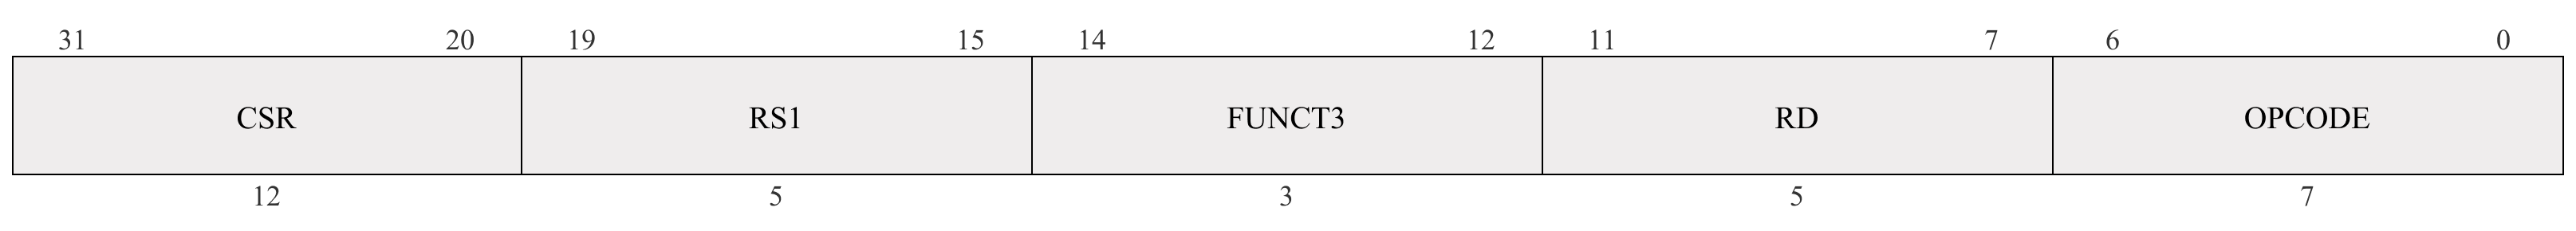
\includegraphics[width=.9\linewidth]{images/csr_instructions.png} } %
  {\scriptsize Source: \href{https://drive.google.com/file/d/1uviu1nH-tScFfgrovvFCrj7Omv8tFtkp/view}{\textit{RISC-V} Unprivileged Manual, page $46$}}
  \caption{Control and Status Register instructions encoding}
  \label{fig:csrinstr}
\end{figure}

Table \ref{tab:csrop} depicts whether a CSR is read or written by every
operation.

\begin{table}
  \centering
  \begin{tabular}{|c|c|c|c|c|}
    \hline
    \textbf{Instruction} & \textbf{Destination reg is x0} & \textbf{Source reg is x0} & \textbf{Reads CSR} & \textbf{Writes CSR} \\
    \hhline{=====} CSRRW & Yes                            & -                         & No                 & Yes                 \\
    \hline
    CSRRW                & No                             & -                         & Yes                & Yes                 \\
    \hline
    CSRRS/CSRRC          & -                              & Yes                       & Yes                & No                  \\
    \hline
    CSRRS/CSRRC          & -                              & No                        & Yes                & Yes                 \\
    \hline
  \end{tabular}
  \caption{CSR operation outcome}
  \label{tab:csrop}
\end{table}

Out of all the CSRs, only a few will be described in the following sections
since they will be necessary to understand the functioning of this project.

\subsection{Machine Status Register (MSTATUS) CSR}
\label{subsec:mstatus}

The \textit{mstatus} register keeps track of and controls the \textit{hart}'s current
operating state. This register will be used to manage interrupts and privilege
levels. Figure \ref{fig:mstatus} depicts a representation of the \textit{mstatus}
CSR.

\begin{figure}[htbp]
  \centering
  \def\stackalignment{r}\stackunder{ 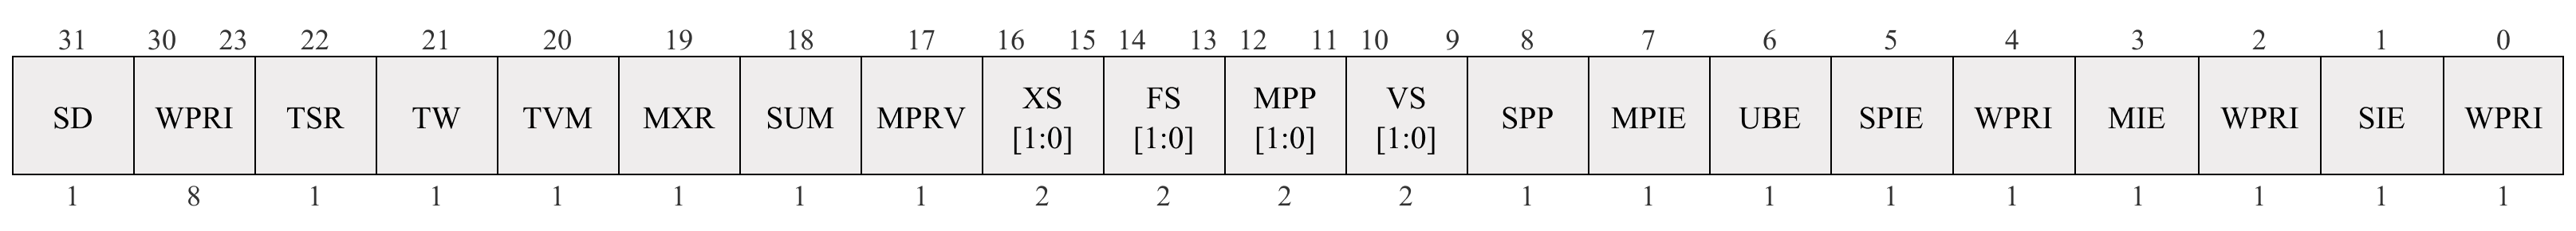
\includegraphics[width=.9\linewidth]{images/mstatus_csr.png} } %
  {\scriptsize Source: \href{https://drive.google.com/file/d/17GeetSnT5wW3xNuAHI95-SI1gPGd5sJ_/view}{\textit{RISC-V} Privileged Manual, page $25$}}
  \caption{Machine Status Register (\textit{mstatus})}
  \label{fig:mstatus}
\end{figure}

Each field in \textit{mstatus} is used to control a specific function of the ISA.
Specifically, the fields are:
\begin{itemize}
  \item Global interrupt-enable bits \textit{MIE} and \textit{SIE} are used to enable
    and disable interrupts for M-mode and S-mode respectively. When a \textit{hart}
    is executing in privilege mode \textit{x}, interrupts are globally enabled when
    $\textit{xIE}= 1$ and globally disabled when $\textit{xIE}= 0$. Interrupts
    for privilege modes \textit{w}, where $\textit{w}< \textit{x}$ are always
    globally disabled regardless of any \textit{wIE} bit set. Interrupts for
    privilege modes \textit{y}, where $\textit{y}> \textit{x}$ are always
    globally enabled regardless of any \textit{yIE} bit set;

  \item \textit{SPIE}, \textit{MPIE}, \textit{SPP}, and \textit{MPP} are used
    when managing a trap. \textit{SPIE} and \textit{MPIE} hold the previous interrupt
    enable bit for S-mode and M-mode respectively. \textit{SPP} and \textit{MPP}
    hold the previous privilege level for S-mode and M-mode respectively. These bits
    are used to track the status of the machine prior to the trap and are necessary
    to correctly restore the context before returning from a trap;

  \item The modify privilege bit \textit{MPRV} modifies the effective privilege
    mode. When $\textit{MPRV}= 0$ loads and store behave normally while, if
    $\textit{MPRV}= 1$ load and store memory addresses are translated and
    protected;

  \item The make executable readable \textit{MXR} bit modifies the privilege
    with which loads access virtual memory. When $\textit{MXR}=0$, only loads
    from pages marked readable will succeed. When $\textit{MXR}=1$, loads from
    pages marked either readable or executable will succeed;

  \item The supervisor user memory access \textit{SUM} bit modifies the
    privilege with which S-mode loads and stores access virtual memory. When $\textit
    {SUM}=0$, S-mode memory accesses to pages that are accessible by U-mode will
    fault. When $\textit{SUM}=1$, these accesses are permitted;

  \item The trap virtual memory \textit{TVM} bit supports intercepting
    supervisor virtual-memory management operations. When $\textit{TVM}=1$,
    attempts to read or write the \textit{satp} CSR while executing in S-mode will
    raise an illegal-instruction exception. When $\textit{TVM}=0$, these operations
    are permitted in S-mode;

  \item The timeout wait \textit{TW} bit supports intercepting the WFI
    instruction. When $\textit{TW}=0$, the WFI instruction may execute in lower
    privilege modes. When $\textit{TW}=1$, then if WFI is executed in any less-privileged
    mode and it does not complete within a time limit, the WFI instruction causes
    an illegal-instruction exception;

  \item The trap sret \textit{TSR} bit supports intercepting the supervisor
    exception return instruction, \textit{SRET}. When $\textit{TSR}=1$, attempts
    to execute \textit{SRET} while executing in S-mode will raise an illegal-instruction
    exception. When $\textit{TSR}=0$, this operation is permitted in S-mode;

  \item The \textit{FS}, \textit{VS}, and the \textit{XS} fields are used to
    reduce the cost of context save and restore by setting and tracking the
    current state of the floating-point unit and any other user-mode extensions
    respectively.
\end{itemize}

\subsection{Machine Exception Program Counter (MEPC) CSR}
\label{subsec:mepc}

The \textit{mepc} register is used, when a trap is taken in M-mode, to store the
address of the instruction that was interrupted or that encountered the
exception. Figure \ref{fig:mepc} depicts a representation of \textit{mepc}.

\begin{figure}[htbp]
  \centering
  \def\stackalignment{r}\stackunder{ 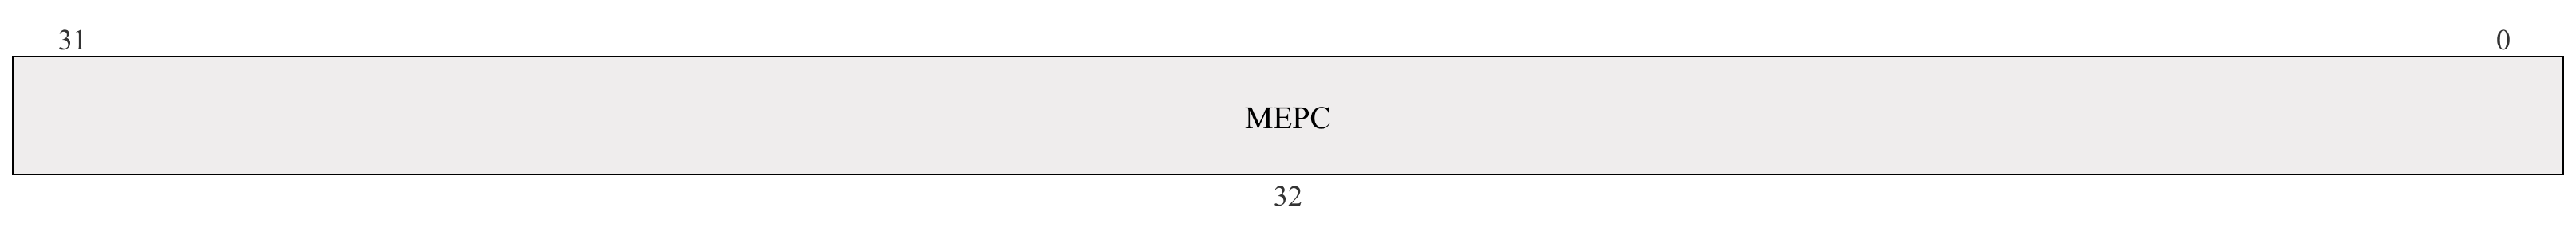
\includegraphics[width=.9\linewidth]{images/mepc_csr.png} } %
  {\scriptsize Source: \href{https://drive.google.com/file/d/17GeetSnT5wW3xNuAHI95-SI1gPGd5sJ_/view}{\textit{RISC-V} Privileged Manual, page $42$}}
  \caption{Machine Exception Program Counter (\textit{mepc})}
  \label{fig:mepc}
\end{figure}

\subsection{Machine Cause Register (MCAUSE) CSR}
\label{subsec:mcause}

The \textit{mcause} register is used, when a trap is taken in M-mode, to store the
code that indicates the event that caused the trap. All the possible codes can
be seen in Table \ref{tab:causes}. Figure \ref{fig:mcause} depicts a representation
of \textit{mcause}.

\begin{figure}[htbp]
  \centering
  \def\stackalignment{r}\stackunder{ 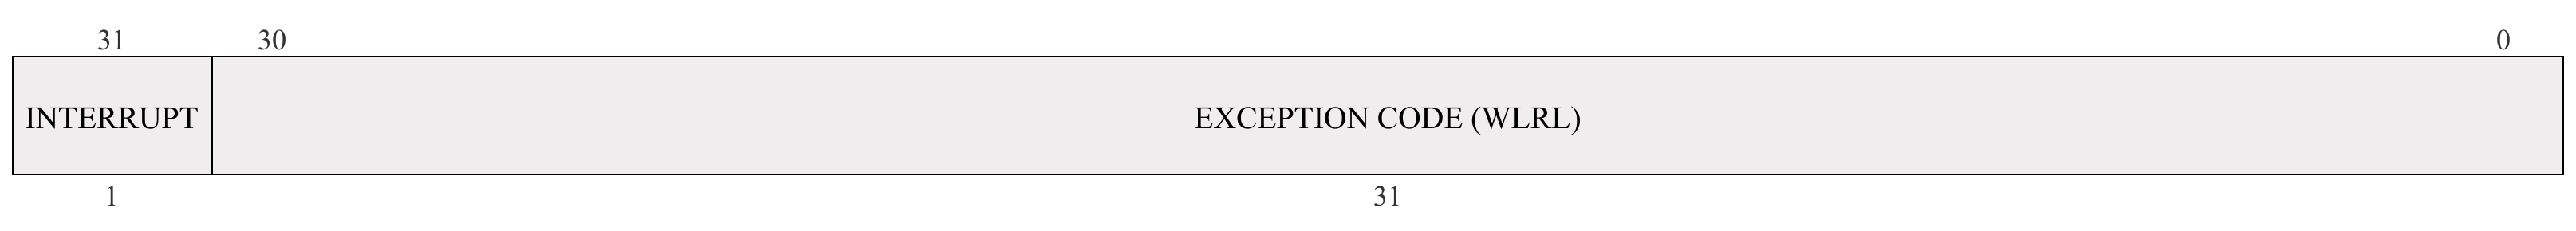
\includegraphics[width=.9\linewidth]{images/mcause_csr.png} } %
  {\scriptsize Source: \href{https://drive.google.com/file/d/17GeetSnT5wW3xNuAHI95-SI1gPGd5sJ_/view}{\textit{RISC-V} Privileged Manual, page $42$}}
  \caption{Machine Cause Register (\textit{mcause})}
  \label{fig:mcause}
\end{figure}

\begin{table}
  \centering
  \begin{tabular}{|c|c|c|}
    \hline
    \textbf{Interrupt} & \textbf{Code} & \textbf{Description}           \\
    \hhline{===} 1     & 0             & User software interrupt        \\
    \hline
    1                  & 1             & Supervisor software interrupt  \\
    \hline
    1                  & 2             & Reserved                       \\
    \hline
    1                  & 3             & Machine software interrupt     \\
    \hline
    1                  & 4             & User timer interrupt           \\
    \hline
    1                  & 5             & Supervisor timer interrupt     \\
    \hline
    1                  & 6             & Reserved                       \\
    \hline
    1                  & 7             & Machine timer interrupt        \\
    \hline
    1                  & 8             & User external interrupt        \\
    \hline
    1                  & 9             & Supervisor external interrupt  \\
    \hline
    1                  & 10            & Reserved                       \\
    \hline
    1                  & 11            & Machine external interrupt     \\
    \hline
    1                  & 12            & Reserved                       \\
    \hline
    1                  & 13            & Counter-overflow interrupt     \\
    \hline
    1                  & 14-15         & Reserved                       \\
    \hline
    1                  & $\geq 16$     & Designated for platform use    \\
    \hhline{===} 0     & 0             & Instruction address misaligned \\
    \hline
    0                  & 1             & Instruction access fault       \\
    \hline
    0                  & 2             & Illegal instruction            \\
    \hline
    0                  & 3             & Breakpoint                     \\
    \hline
    0                  & 4             & Load address misaligned        \\
    \hline
    0                  & 5             & Load access fault              \\
    \hline
    0                  & 6             & Store/AMO address misaligned   \\
    \hline
    0                  & 7             & Store/AMO access fault         \\
    \hline
    0                  & 8             & Environment call from U-mode   \\
    \hline
    0                  & 9             & Environment call from S-mode   \\
    \hline
    0                  & 10            & Reserved                       \\
    \hline
    0                  & 11            & Environment call from M-mode   \\
    \hline
    0                  & 12            & Instruction page fault         \\
    \hline
    0                  & 13            & Load page fault                \\
    \hline
    0                  & 14            & Reserved                       \\
    \hline
    0                  & 15            & Store/AMO page fault           \\
    \hline
    0                  & 16-17         & Reserved                       \\
    \hline
    0                  & 18            & Software check                 \\
    \hline
    0                  & 19            & Hardware check                 \\
    \hline
    0                  & 20-23         & Reserved                       \\
    \hline
    0                  & 24-31         & Designated for custom use      \\
    \hline
    0                  & 32-47         & Reserved                       \\
    \hline
    0                  & 48-63         & Designated for custom use      \\
    \hline
    0                  & $\geq 64$     & Designated for custom use      \\
    \hline
  \end{tabular}
  \caption{Interrupts and Exception causes}
  \label{tab:causes}
\end{table}

\subsection{Machine Trap Value Register (MTVAL) CSR}
\label{subsec:mtval}

The \textit{mtval} register is used, when a trap is taken in M-mode, to store
exception-specific information to assist software in handling the trap. Figure \ref{fig:mcause}
depicts a representation of \textit{mtval}.

\begin{figure}[htbp]
  \centering
  \def\stackalignment{r}\stackunder{ 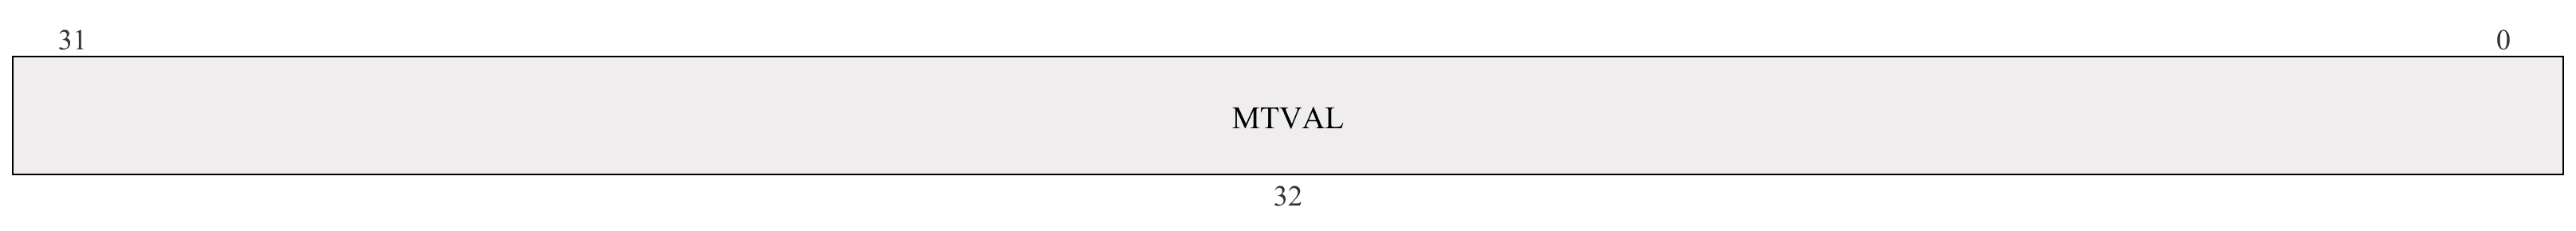
\includegraphics[width=.9\linewidth]{images/mtval_csr.png} } %
  {\scriptsize Source: \href{https://drive.google.com/file/d/17GeetSnT5wW3xNuAHI95-SI1gPGd5sJ_/view}{\textit{RISC-V} Privileged Manual, page $45$}}
  \caption{Machine Trap Value Register (\textit{mtval})}
  \label{fig:mtval}
\end{figure}

\subsection{Machine Trap-Vector Base-Address Register (MTVEC) CSR}
\label{subsec:mtvec}

The \textit{mtvec} register is used to store the address that holds the trap vector
configuration. Figure \ref{fig:mtvec} depicts a representation of \textit{mtvec}.
The \textit{MODE} field can be set according to Table \ref{tab:mode}. If we set
the \textit{MODE} to vectored, all asynchronous interrupts will set the program
counter to the base address encoded in \textit{mtvec} plus $4$ times the cause of
the interrupt (causes can be seen in Table \ref{tab:causes}). With \textit{MODE}
set to direct instead, all traps set the program counter to the base address.

\begin{figure}[htbp]
  \centering
  \def\stackalignment{r}\stackunder{ 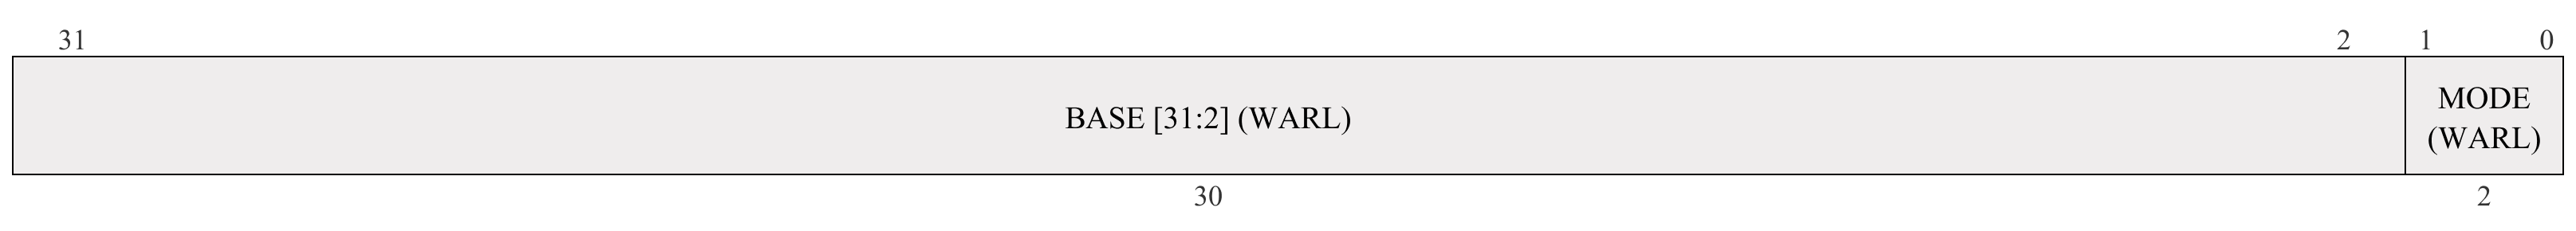
\includegraphics[width=.9\linewidth]{images/mtvec_csr.png} } %
  {\scriptsize Source: \href{https://drive.google.com/file/d/17GeetSnT5wW3xNuAHI95-SI1gPGd5sJ_/view}{\textit{RISC-V} Privileged Manual, page $34$}}
  \caption{Machine Trap-Vector Base-Address Register (\textit{mtvec})}
  \label{fig:mtvec}
\end{figure}

\begin{table}
  \centering
  \begin{tabular}{|c|c|c|}
    \hline
    \textbf{Value}   & \textbf{Name} & \textbf{Description}                                                      \\
    \hhline{===} $0$ & Direct        & All traps set $\textit{pc}= \textit{BASE}$                                \\
    \hline
    $1$              & Vectored      & Asynchronous interrupts set $\textit{pc}= \textit{BASE}+4*\textit{cause}$ \\
    \hline
    $\geq 2$         & -             & Reserved                                                                  \\
    \hline
  \end{tabular}
  \caption{Encoding of \textit{MODE} for \textit{mtvec} register}
  \label{tab:mode}
\end{table}

\subsection{ (MIDELEG) CSR}
\label{subsec:mideleg}

\subsection{ (MEDELEG) CSR}
\label{subsec:medeleg}

\section{RISC-V Physical Memory Protection (PMP)}
\label{sec:riscv_pmp}

\textit{RISC-V} provides an optional Physical Memory Protection (PMP) unit that
allows to configure access privileges (read, write, and execute) for each
physical memory region. The PMP ensures secure processing and helps to contain faults.

PMP checks are applied at all accesses in S or U mode. Optionally, PMP checks may
additionally apply to M-mode accesses, in which case the PMP registers
themselves are locked, so that even M-mode software cannot change them until the
hart is reset. Each PMP check results either in a violation which is trapped at
the processor or in a granted permission.

\subsection{PMP CSRs}
\label{subsec:riscv_pmpcsr}

Each PMP entry is described by an 8-bit configuration register (\textit{pmpXcfg})
and one $32$-bit address register (\textit{pmpaddrX}). Sixteen CSRs, \textit{pmpcfg0-pmpcfg15},
hold the configurations \textit{pmp0cfg-pmp63cfg} for the 64 PMP entries (as shown
in Figure \ref{fig:pmpcfgs}). Each PMP address (\textit{pmpaddr0-pmpaddr63})
encodes bits $33$-$2$ of a $34$-bit physical address as shown in Figure
\ref{fig:pmpaddr}.

Each PMP configuration register (Figure \ref{fig:pmpconf}) contains:
\begin{itemize}
  \item R-bit: when set allows read access;

  \item W-bit: when set allows write access;

  \item X-bit: when set allows instruction execution;

  \item A-bits: used to set address matching mode (better explained in subsection
    \ref{subsec:pmpaddressmatching});

  \item L-bit: when set the configuration is locked, meaning that it can't be modified
    without a system reset.
\end{itemize}

\begin{figure}[htbp]
  \centering
  \def\stackalignment{r}\stackunder{ 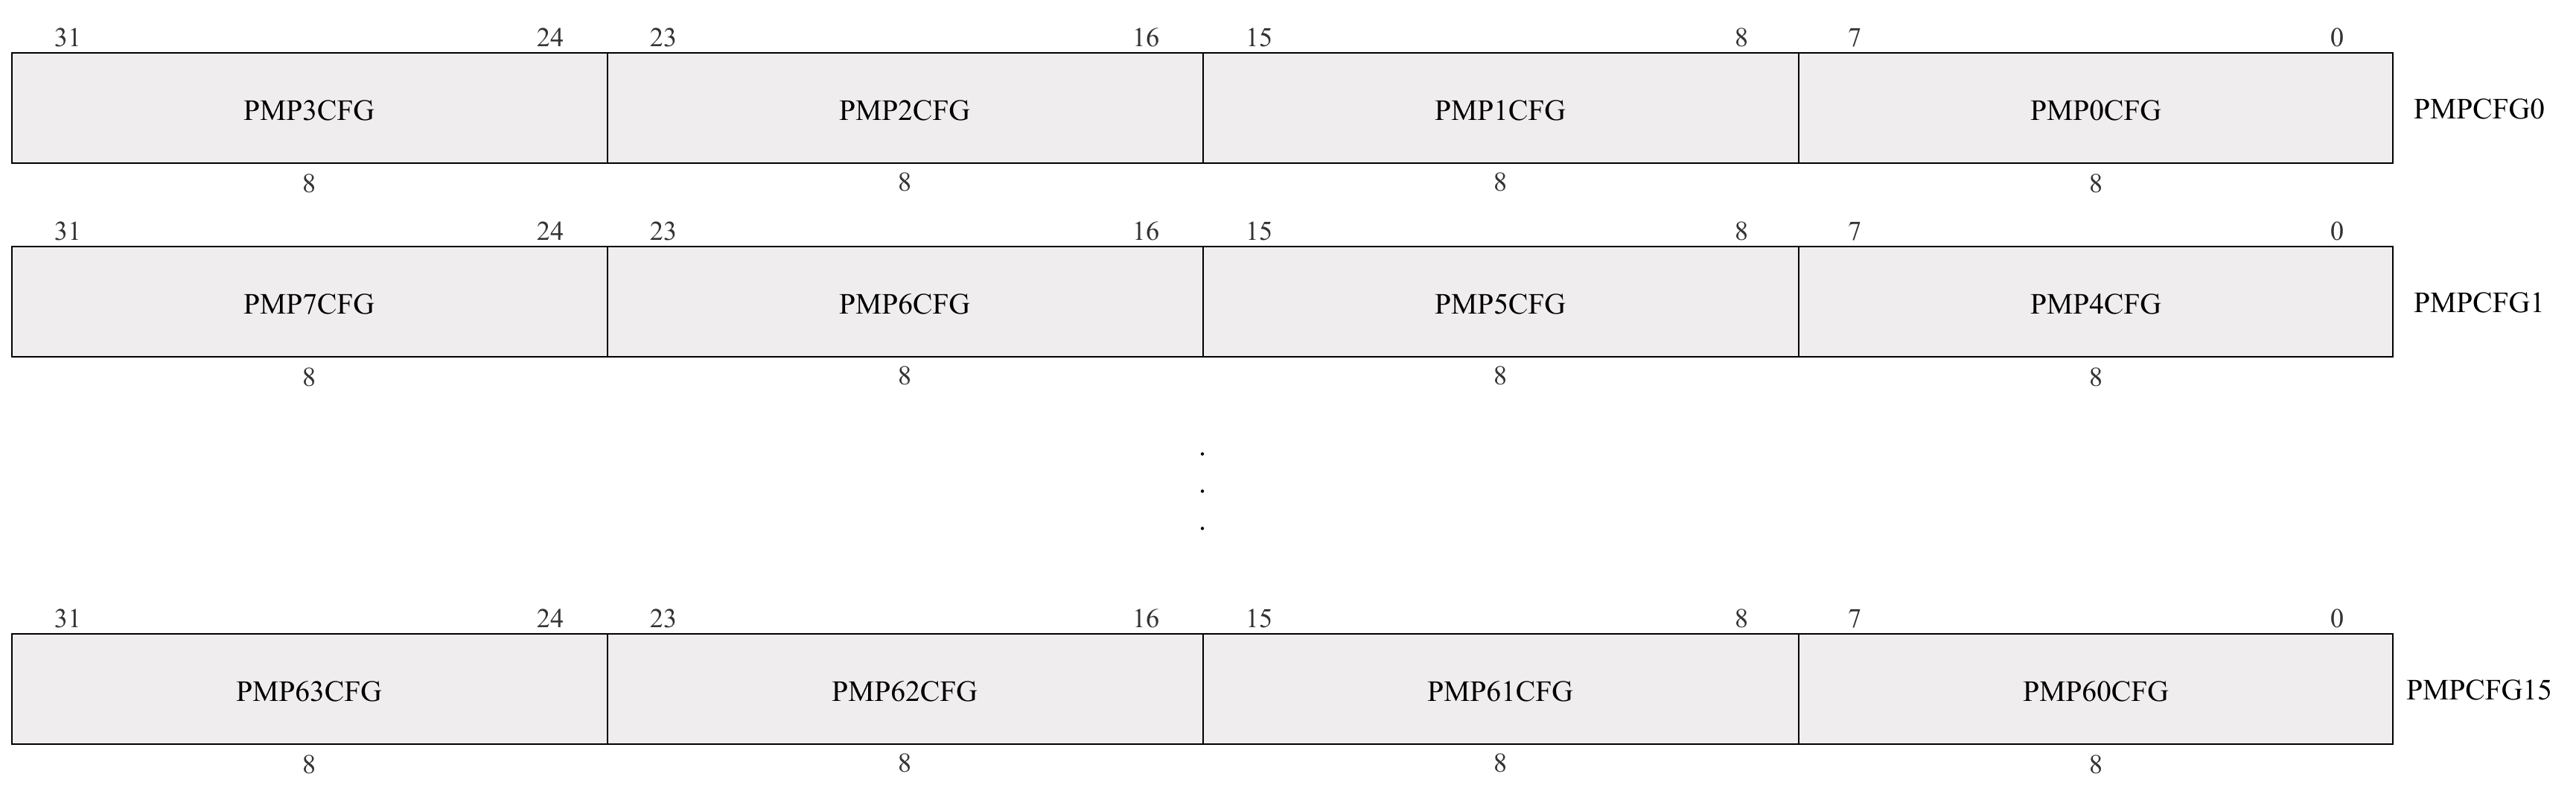
\includegraphics[width=.9\linewidth]{images/pmpcfgs_csr.png}}
  {\scriptsize Source: \href{https://drive.google.com/file/d/17GeetSnT5wW3xNuAHI95-SI1gPGd5sJ_/view}{\textit{RISC-V} Privileged Manual, page $60$}}
  \caption{PMP Configuration CSR (\textit{pmpcfg0-pmpcfg15})}
  \label{fig:pmpcfgs}
\end{figure}

\begin{figure}[htbp]
  \centering
  \def\stackalignment{r}\stackunder{ 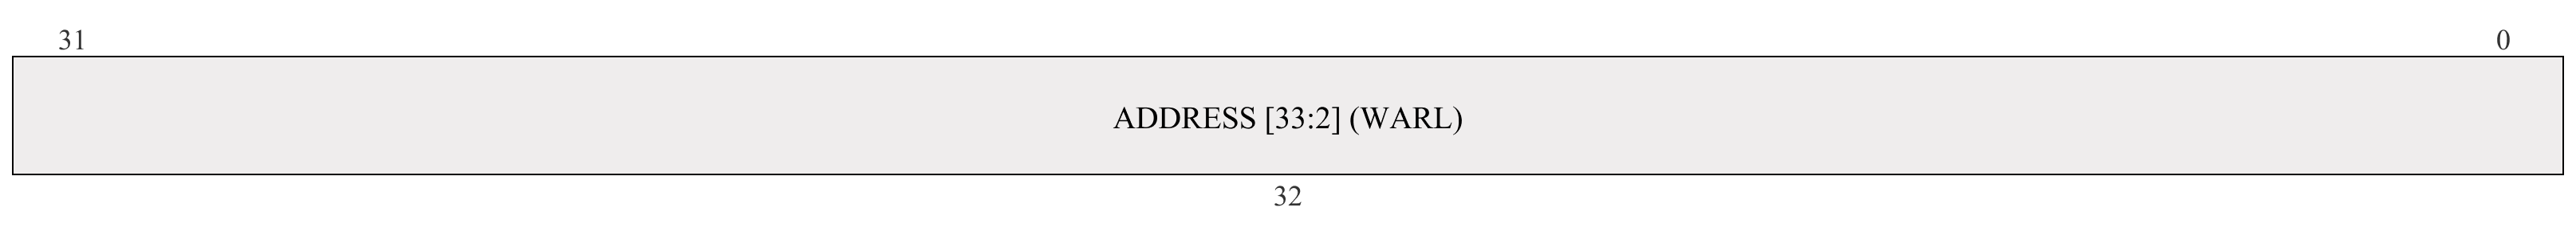
\includegraphics[width=.9\linewidth]{images/pmpaddress_csr.png} } %
  {\scriptsize Source: \href{https://drive.google.com/file/d/17GeetSnT5wW3xNuAHI95-SI1gPGd5sJ_/view}{\textit{RISC-V} Privileged Manual, page $61$}}
  \caption{PMP Address CSR (\textit{pmpaddr})}
  \label{fig:pmpaddr}
\end{figure}

\begin{figure}[htbp]
  \centering
  \def\stackalignment{r}\stackunder{ 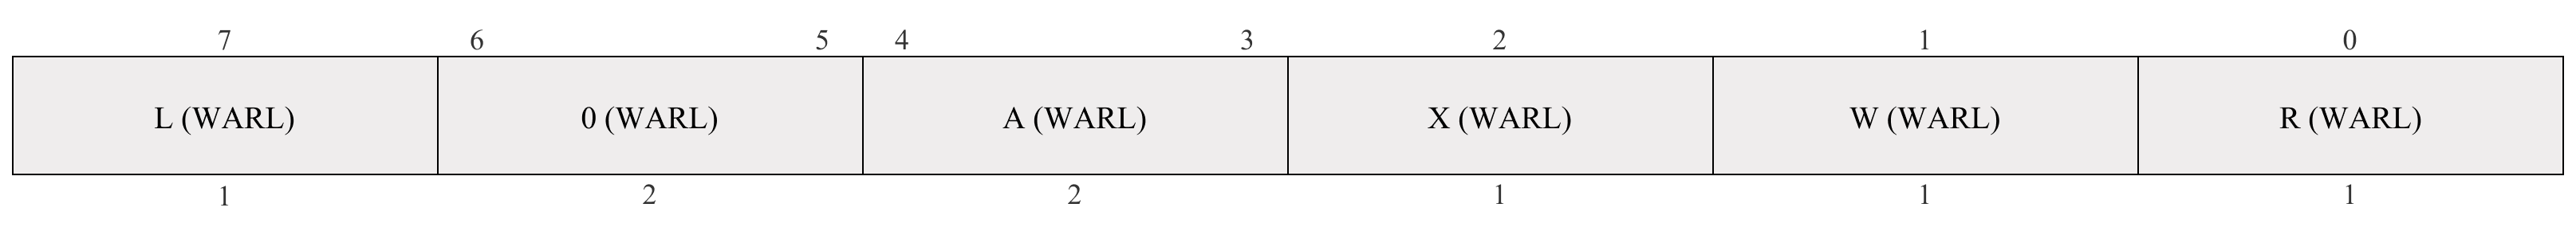
\includegraphics[width=.9\linewidth]{images/pmpconf_csr.png} } %
  {\scriptsize Source: \href{https://drive.google.com/file/d/17GeetSnT5wW3xNuAHI95-SI1gPGd5sJ_/view}{\textit{RISC-V} Privileged Manual, page $61$}}
  \caption{PMP Configuration Register Format}
  \label{fig:pmpconf}
\end{figure}

\subsection{PMP Address Matching}
\label{subsec:pmpaddressmatching}

The A field in a PMP entry's configuration register encodes the address-matching
mode of the associated PMP address register (encoding shown in Table \ref{tab:addressmatching}).

\begin{table}
  \centering
  \begin{tabular}{|c|c|c|}
    \hline
    \textbf{A}       & \textbf{Name} & \textbf{Description}                  \\
    \hhline {===} 00 & OFF           & Null region (disabled)                \\
    \hline
    01               & TOR           & Top of range                          \\
    \hline
    10               & NA4           & Naturally aligned four-byte region    \\
    \hline
    11               & NAPOT         & Naturally aligned power-of-two region \\
    \hline
  \end{tabular}
  \caption{Encoding of A field in PMP Configuration Register}
  \label{tab:addressmatching}
\end{table}

When $A=0$, this PMP entry is disabled and matches no addresses. Two other address-matching
modes are supported:
\begin{itemize}
  \item Naturally aligned power-of-$2$ regions (NAPOT): NAPOT ranges make use of
    the low-order bits of the associated address register to encode the size of
    the range. This includes the special case of naturally aligned four-byte regions
    (NA4);

  \item Top boundary of an arbitrary range (TOR): If TOR is selected, the associated
    address register forms the top of the address range, and the preceding PMP
    address register forms the bottom of the address range. Note that, if the
    first PMP address is configured as TOR the lower boundary is considered to
    be \textit{0x0}.
\end{itemize}

\subsection{PMP Matching Logic}
\label{subsec:matchinglogic}

PMP entries are statically prioritized. The lowest-numbered PMP entry that matches
any byte of an access determines whether that access succeeds or fails. The
matching PMP entry must match all bytes of an access, or the access fails,
irrespective of the L, R, W, and X bits. For example, if a PMP entry is configured
to match the four-byte range \textit{0xC-0xF}, then an $8$-byte access to the range
\textit{0x8-0xF} will fail, assuming that such PMP entry is the highest-priority
entry that matches those addresses.

If a PMP entry matches all bytes of an access, then the L, R, W, and X bits determine
whether the access succeeds or fails. If the L bit is clear and the privilege
mode of the access is M, the access succeeds. Otherwise, if the L bit is set or the
privilege mode of the access is S or U, then the access succeeds only if the R, W,
or X bit corresponding to the access type is set.

If no PMP entry matches an S-mode or U-mode access, but at least one PMP entry is
implemented, the access fails. Failed accesses generate a load, store, or instruction
access exception.
  \chapter{Control Flow Integrity Enforcer}
\label{cha:project}

This chapter focuses on \textit{project name}'s implementation. We will see the
goals and specifics of the project as well as a detailed description of every
key aspect of the development. Lastly, a Proof of Concept is discussed to prove
the functioning and security capabilities of \textit{project name}.

\section{Project Formalization}
\label{sec:project_formalization}

This project aims at providing a secure infrastructure for embedded devices
based on the \textit{RISC-V} ISA. The main goal is to protect the device from
control-flow attacks such as Return-Oriented Programming (ROP) attacks. To do so,
\textit{project name} provides a Control Flow Integrity (CFI) Enforcer which ensures
that the software follows the expected path. Moreover, it provides instrumenting
capabilities to automatize the implementation of any code.

Control Flow Integrity is a security technique that does not allow control transfers
that are not part of the Control Flow Graph (CFG) of the binary.

Another goal of this project is to be as lightweight as possible to meet the performance
requirements of less powerful devices. Thus, great importance is given to optimization
of both space and time consumption.

\textit{project name} makes it possible to run untrusted code in a secure
environment protecting the execution path of the software and ensures that any
attack attempt will be detected by the CFI Enforcer and thus, the device will not
be compromised.

This project makes use of \textit{RISC-V} capabilities like the PMP to implement
secure spaces of memory. It also utilizes state-of-the-art solutions like a Shadow
Stack and a Control Flow Graph to ensure the correctness of the policies.

\section{Project Specifics}
\label{sec:project_specifics}

\begin{wrapfigure}
  {l}{.25\textwidth}
  \centering
  \def\stackalignment{l}\stackunder{ 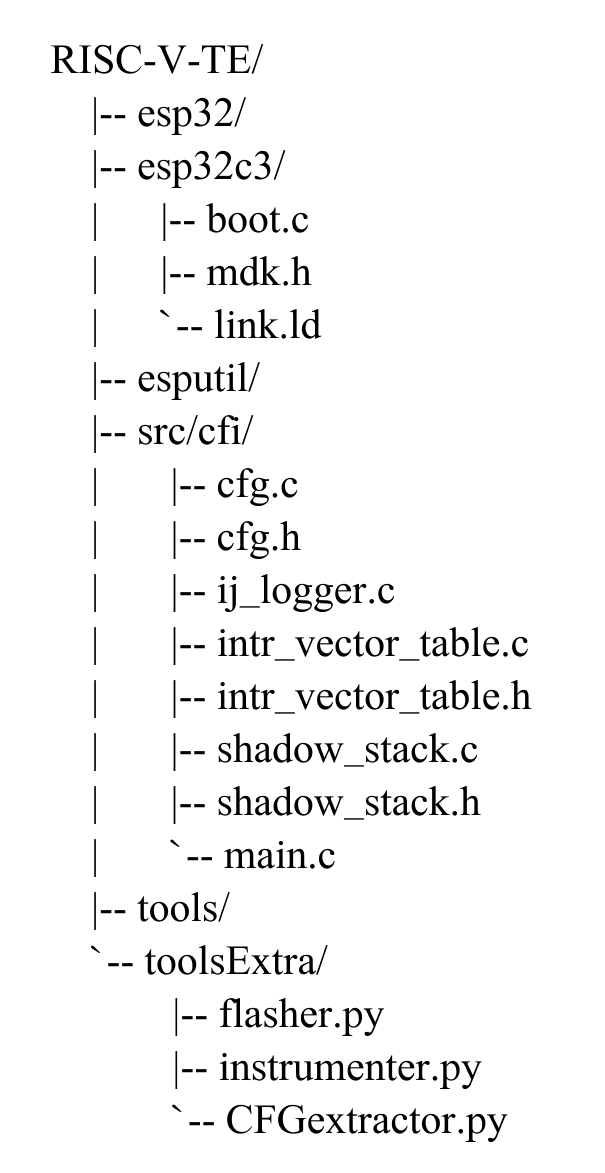
\includegraphics[width=\linewidth]{images/workingtree.png} } %
  {\scriptsize }
  \caption{Working Tree}
  \label{fig:workingtree}
\end{wrapfigure}

The project has been developed on \textit{Espressif's ESP32-C3-DevKitM-1}
\cite{esp32c3} and the basic configuration for bare-metal flashing on such board
is derived by Sergey Lyubka's project \textit{mdk}\cite{mdk}. Lastly, the
\textit{riscv-none-elf}\cite{toolchain} toolchain has been used to cross-compile
the code. However, since the project has been developed following the ideas of
\textit{RISC-V} about hardware abstraction any of these settings can be modified
according to one needs\footnote{Note that if we wish to change the target board,
all vendor-specific files needed to flash the code must replace \textit{Espressif}'s
files}.

Figure \ref{fig:workingtree} depicts the working tree of the project, where:
\begin{itemize}
  \item \textit{esp32} contains the boot configuration and linker script for
    general \textit{Espressif}'s boards;

  \item \textit{esp32c3} contains the boot configuration and linker script for
    the \textit{ESP32-C3};

  \item \textit{esputil} contains \textit{Espressif}'s utils used to manage the board;

  \item \textit{src/cfi/usercode} contains the untrusted code that needs
    protection during execution. The code inside this folder will be the target for
    code instrumentation;

  \item \textit{src/cfi} contains the source files for the Shadow Stack, Control
    Flow Graph, interrupt vector table and machine setup;

  \item \textit{toolsExtra} contains the Python scripts used to instrument, build,
    and flash the code.
\end{itemize}

The scripts inside \textit{toolsExtra} are used to compile, instrument, and run
the code (detailed description in Section \ref{sec:project_instrumentation}). Moreover,
the file \textit{CFGextractor.py} is used to extract the Control Flow Graph of the
code.

Inside \textit{src/cfi} instead, we find the code responsible for managing the machine
mode operations. File \textit{main.c} is responsible for setting up interrupts,
managing privilege modes, and setting up both the PMP (detailed description in
Section \ref{sec:project_pmp}) and the interrupt vector table (detailed
description in Section \ref{sec:project_isr}). File \textit{intr\_vector\_table.c}
is responsible for managing interrupts and exceptions as well as performing controls
on both forward and backward checks (detailed description in Section
\ref{sec:project_controls}). Files \textit{cfg.c} and \textit{shadow\_stack.c}
hold the Control Flow Graph and the Shadow Stack configurations respectively (detailed
description in Sections \ref{sec:project_cfg} and \ref{sec:project_ss}). Lastly,
\textit{ij\_logger.c} is used to retrieve indirect jump addresses thanks to a logger.

\section{Code Instrumentation}
\label{sec:project_instrumentation}

Code instrumentation is the process of modifying software (usually binary or assembly
code) by inserting instructions to perform specific tasks such as a performance
analysis. Instrumentation plays a critical role in this project as it allows to modify
the untrusted code in a simple yet effective way. Moreover, this automatize the process
leading to faster development and lower number of errors. The whole
instrumentation procedure is depicted in Figure \ref{fig:instrumentation}.

\begin{figure}[htbp]
  \centering
  \def\stackalignment{r}\stackunder{ 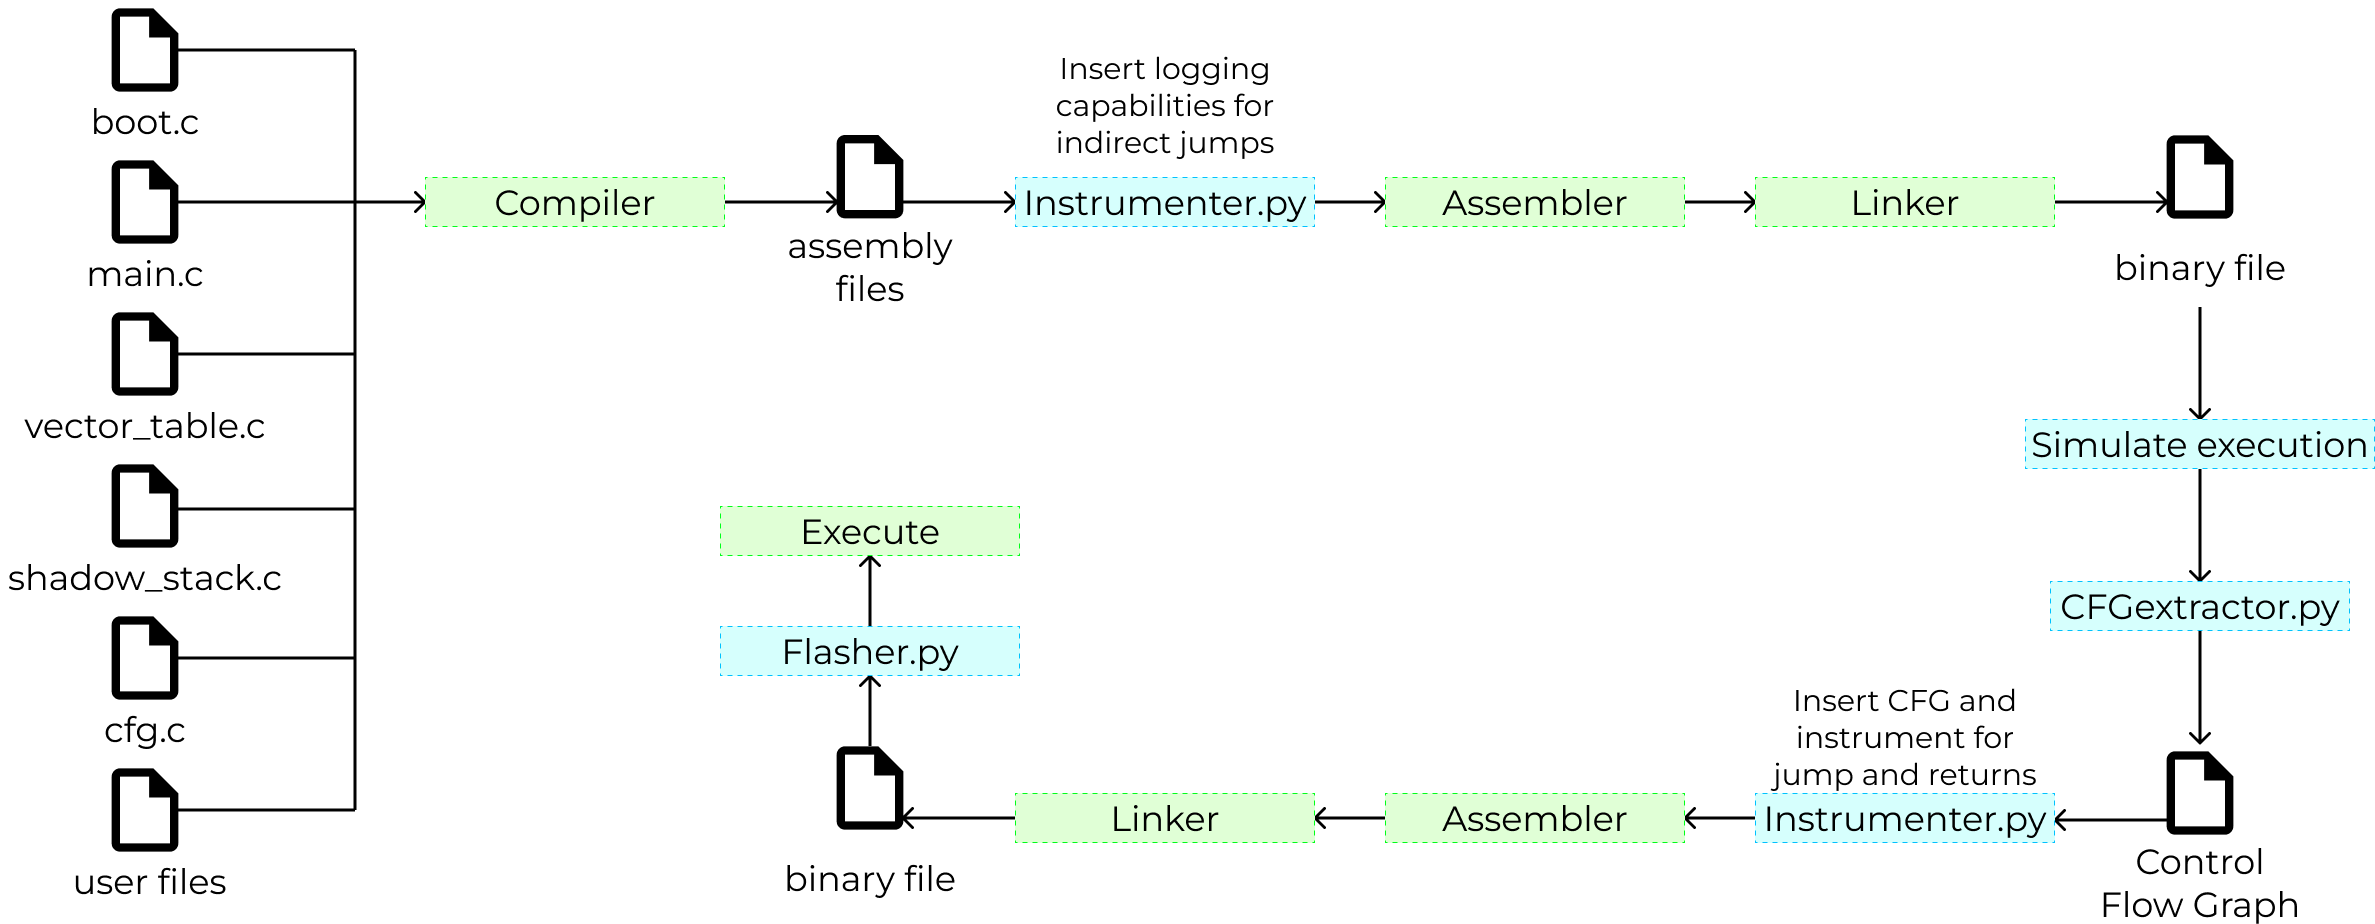
\includegraphics[width=.9\linewidth]{images/instrumentation.png} } %
  {\scriptsize }
  \caption{Flow of the Code Instrumentation Procedure}
  \label{fig:instrumentation}
\end{figure}

The script \textit{flasher.py} can be run with the command \textit{python3
flasher.py [command]}, where \textit{command} can be:
\begin{itemize}[noitemsep]
  \item \textit{build}: for building the source files and producing the binary;

  \item \textit{run}: for building and running the binary on the target device;

  \item \textit{clear}: for clearing output files in the directory;

  \item \textit{secure-build}: for instrumenting and building the source files and
    producing the secure binary;

  \item \textit{secure-run}: for instrumenting, building, and running the secure
    binary on the target device.
\end{itemize}

As we can see the instrumentation only happens with \textit{secure-build} and
\textit{secure-run} commands. Normal building and running commands have been
implemented to make a comparison between an untrusted code and the trusted one.

\subsection{Instrumentation for logging}
\label{subsec:logging}

If we run \textit{flasher.py} with \textit{secure} commands the instrumentation phase
follows the steps described below.

All source files are compiled into assembly files with the toolchain, then the
untrusted user files are passed to \textit{instrumenter.py}. Firstly, the code is
instrumented with logging capabilities to retrieve indirect jump destinations.
This is done by searching indirect jump instruction (\textit{JALR}) with the regex
\textit{$\backslash$b(jalr)$\backslash$b$\backslash$s+($\backslash$w+)} which
retrieves any occurrence of \textit{jalr \{register\}}\footnote{Usually the
compiler uses register \textit{a5} for \textit{JALR} instructions.}.

\begin{wrapfigure}
  {r}{0.25\textwidth}
  \setlength{\intextsep}{0pt}
  \begin{minipage}{0.25\textwidth}
    \begin{lstlisting}[style=Assembly, caption = Logging code block, label={lst:loggingblock}]
addi sp,sp,-40
sw a5,4(sp)
sw a4,8(sp)
sw a2,12(sp)
sw a1,16(sp)
sw a0,20(sp)
sw s0,24(sp)
sw s1,28(sp)
sw s2,32(sp)
sw s3,36(sp)
mv a1,{register}
auipc a0,0
addi a0,a0,38
call print_reg
lw a5,4(sp)
lw a4,8(sp)
lw a2,12(sp)
lw a1,16(sp)
lw a0,20(sp)
lw s0,24(sp)
lw s1,28(sp)
lw s2,32(sp)
lw s3,36(sp)
addi sp,sp,40
jalr {register}
    \end{lstlisting}
  \end{minipage}
\end{wrapfigure}

Once we retrieve the source register for the \textit{JALR} instruction we add
the block of code depicted in Listing \ref{lst:loggingblock} before the jump. This
effectively allows us to save the state of the machine and call the function \textit{print\_reg}
passing the destination address and the program counter of the \textit{JALR} instruction
as arguments. The destination address is simply stored in the source register
while the source address is computed by loading the current program counter with
\textit{auipc a0, 0} and by adding $38$\footnote{Note that $38$ is the distance
in Bytes from the instruction that load the \textit{pc} to the \textit{JALR}
instruction.} to it. The \textit{print\_reg} function, when called, will then
print a string like \textit{Source: 0x40380100 - Destination:0x40380200}.

\subsection{Control Flow Graph Extraction}
\label{subsec:project_cfgextraction}

As soon as the first instrumentation is completed, the assembly files are assembled
and linked to produce the binary. If, during instrumentation, we have found that
there are indirect jumps in the code we perform a ``simulation''\footnote{The
simulation consists in running the code on the target device transparently.} of the
execution to retrieve the logging of the \textit{print\_reg} function.

After that \textit{CFGextractor.py} is called to extract the Control Flow Graph of
the user code. The extraction is divided in two phases:
\begin{itemize}
  \item Dynamic phase: in the dynamic phase we parse the output retrieved from
    the simulation to create source-destination pairs of addresses. Note that in
    this phase addresses are also adjusted by removing the size of the logging block
    from their value. This is done because, during the simulation we injected the
    logging block before each jump, thus increasing the size of the binary. For each
    address we count the number of blocks that appeared before it and we compute
    $\textit{final\_address}= \textit{retrieved\_value}- (\textit{block\_size}* \textit
    {block\_number})$;

  \item Static phase: in the static phase we simply parse the dump file obtained
    with \textit{riscv-none-elf-objdump} searching for \textit{JAL} instructions.
    These direct jump are statically defined so we can retrieve them with the dump
    file. Each time a \textit{JAL} instruction is found the pair source-destination
    is added to the CFG.
\end{itemize}

Once the Control Flow Graph is extracted, all the pairs are ordered in ascending
ordered firstly by source and then by destination. This is because with indirect
jump instructions we could have that more destinations could share the same
source. After that, execution is returned to \textit{instrumenter.py}.

\subsection{Instrumentation for forward and backward edge controls}
\label{subsec:project_instrcontrols}

In this last instrumentation phase we need to add code blocks that allows us to
perform forward and backward edge controls. Such blocks must be added before every
direct jump, indirect jump, and return instruction. To do so, we parse the assembly
files, and, search for the target instructions thanks to the regex functions depicted
in Table \ref{tab:regexes}.

\begin{table}
  \centering
  \begin{tabular}{|c|c|}
    \hline
    \textbf{Regex}                                                                      & \textbf{Use}                            \\
    \hhline{==} \textit{$\backslash$b(call)$\backslash$b$\backslash$s+($\backslash$w+)} & Used to find \textit{JAL} instructions  \\
    \hline
    \textit{$\backslash$b(jalr)$\backslash$b$\backslash$s+($\backslash$w+)}             & Used to find \textit{JALR} instructions \\
    \hline
    \textit{$\backslash$b(jr)$\backslash$b$\backslash$s+($\backslash$w+)}               & Used to find \textit{RET} instructions  \\
    \hline
  \end{tabular}
  \caption{Regex functions used to find target instructions}
  \label{tab:regexes}
\end{table}

Depending on the instruction we find during parsing we do the following:
\begin{itemize}
  \item \textit{JAL} instructions: if we find a direct jump instruction we need to
    add the code depicted in Listing \ref{lst:dirjumpblock} before the target.
    This code loads the address of the target function in register \textit{a7} and
    then performs and \textit{ECALL} instruction (detailed functioning explained
    in \ref{sec:project_isr});

  \item \textit{JALR} instructions: if we find an indirect jump instruction we need
    to add the code depicted in Listing \ref{lst:indirjumpblock} before the target.
    This code copies the address stored in the target register into register
    \textit{a7} and then performs and \textit{ECALL} instruction;

  \item \textit{RET} instructions: if we find a return instruction we need to add
    the code depicted in Listing \ref{lst:retblock} before the target. This code
    copies the return address stored in the return address register into
    register \textit{a7} and then performs and \textit{ECALL} instruction. In Section
    \ref{sec:project_isr} we will see why, in this case, we need to add $1$ to the
    return address.
\end{itemize}

\begin{lstlisting}[style=Assembly, caption = Direct jump code block, label={lst:dirjumpblock}]
la a7, {target_function}
ecall
jal {target_function}
\end{lstlisting}

\begin{lstlisting}[style=Assembly, caption = Indirect jump code block, label={lst:indirjumpblock}]
mv a7, {target_register}
ecall
jalr {target_register}
\end{lstlisting}

\begin{lstlisting}[style=Assembly, caption = Return code block, label={lst:retblock}]
addi a7, {return_address_register}, 1
ecall
addi {return_address_register}, a7, -1
ret {return_address_register}
\end{lstlisting}

In the last step of the instrumentation we inject the previously crafted Control
Flow Graph into the \textit{cfg.c} file.

After this second instrumentation ends, the modified assembly files are assembled
and linked by \textit{flasher.py} to produce the secure binary file. Lastly, if
we used the \textit{secure-run} command, the binary file is flashed on the
target device for execution.

\section{Interrupts Service Routine}
\label{sec:project_isr}

In this section, we will see how the interrupt vector table is implemented and
how interrupts and exceptions are handled in this project. Most importantly we will
see how forward and backward edge controls are enforced.

The interrupt vector table is defined inside \textit{intr\_vector\_table.c}. As already
explained its address is loaded in \textit{main.c} and stored inside \textit{mtvec}
(\ref{subsec:mtvec}) with \textit{MODE} set to vectored. This means that every asynchronous
interrupt will set the program counter to the base address of the vector table plus
$4$ times the cause of the interrupt. Any other interrupt and exception is
trapped inside the function \textit{synchronous\_exception\_handler} which redirects
to the correct function depending on the trap cause. Listing \ref{lst:intrtable}
depicts the actual implementation of the interrupt vector table.

Most of the exceptions and interrupts are not currently handled and, when invoked,
they just log a message describing which trap was taken. Afterward, the
execution is resumed. This design choice has been made for two reasons. The
first being that such implementation would be out of scope since we aim at
providing the bare minimum implementation for enforcing Control Flow Integrity. The
second instead is that we do not need those handler and we leave space for implementation-specific
requirements. For example, if an implementation makes use of external interrupts,
the developer would just need to insert the desired handling in the correct
function inside the \textit{intr\_vector\_table.c} file. As explained, this implementation
provides the required security features while leaving space for customization.

Since \textit{ECALLS} are defined as exceptions in \textit{RISC-V}, the
interrupt vector table is responsible for managing them. For this reason, the
only implemented function in the interrupt vector table is the handler for U-mode
\textit{ECALL}s. This implementation is tailored for managing forward and backward
edge controls. However, since \textit{ECALL}s can be used for different purposes
the handler is designed to be expandable. Table \ref{tab:ecalls} depicts the
current allowed ecalls.

\begin{table}
  \centering
  \begin{tabular}{|c|c|c|}
    \hline
    \textbf{Code}                & \textbf{Use}     & \textbf{Description}                  \\
    \hhline{===} $1$             & Reserved         & Used to terminate execution           \\
    \hline
    \textit{destination address} & Forward control  & Used to check the destination address \\
    \hline
    $\textit{return address}+ 1$ & Backward control & Used to check the return address      \\
    \hline
  \end{tabular}
  \caption{Encoding of current Ecall values}
  \label{tab:ecalls}
\end{table}

\begin{lstlisting}[style=CStyle, caption = Interrput Vector Table, label={lst:intrtable}]
void interrupt_vector_table(void) {
  asm volatile("j synchronous_exception_handler");
  asm volatile("j isr_supervisor_software");
  asm volatile("j isr_reserved");
  asm volatile("j isr_machine_software");
  asm volatile("j isr_user_timer");
  asm volatile("j isr_supervisor_timer");
  asm volatile("j isr_reserved");
  asm volatile("j isr_machine_timer");
  asm volatile("j isr_user_external");
  asm volatile("j isr_supervisor_external");
  asm volatile("j isr_reserved");
  asm volatile("j isr_machine_external");
  asm volatile("j isr_reserved");
}
\end{lstlisting}

Currently, the U-mode \textit{ECALL} handler is implemented as depicted in
Listing \ref{lst:ecallhandler}. As it is possible to see we encoded the \textit{ECALL}
code and the address required for control integrity checks into a single value. This
design has been used to minimize the use of registers. Another solution would
have been to use a register, say \textit{a7}, to hold the \textit{ECALL} code, and
another register, say \textit{a6}, to hold the address to check. However, since
legal addresses must be even we can encode in one register both the value of the
\textit{ECALL} code and the address (Figure \ref{fig:ecall} shows the encoding
of register \textit{a7}). When the interrupt vector table needs to check which code
is used we can just see if the value in \textit{a7}\footnote{In Listing
\ref{lst:ecallhandler} register \textit{a7} is represented by the parameter \textit{ecode}.}
is even or odd and, depending on the result we can decide which operation to
perform (even values will lead to a forward edge check while odd values will lead
to a backward edge check). When we need to check for a return address we first subtract
$1$ from it to obtain the original value of the address and then we perform the control.

Note that the use of register \textit{a7} to hold \textit{ECALL} codes is purely
a design choice and, to ensure that such register is not tampered with by the
compiler it has been ``disabled'', meaning that the compiler will never use such
register. This choice allows us to be sure that only the interrupt vector table
and the code blocks that we inject modify the value of \textit{a7}.

If one wish to add a new custom \textit{ECALL} code for other purposes he just
need to put a control before the code checks if the code is even or not. Say that
we want to add code $2$ to perform a specific operation. To do so, we just need to
add a check like \textit{else if(ecode == 2) \{perform operation\}} after the
first check, if the check fails the code will eventually check if the code is even
or not and perform the corresponding control.

It is easy to see how this implementation effectively addresses the problem and does
not suffer from possible future customization of the interrupt vector table.

\begin{lstlisting}[style=CStyle, caption = U-mode \textit{ECALL} handler, label={lst:ecallhandler}]
void esr_handler_U_mode_ecall(u_int ecode, u_int mepc)
{
  if (ecode == 1)
  {
    // Terminate execution
  }
  else if ((ecode % 2) == 0)
  {
    // Forward edge control
  }
  else if ((ecode % 2) != 0)
  {
    // Backward edge control
  } else
  {
    // Undefined ecall code
  }
}
\end{lstlisting}

\begin{figure}[htbp]
  \centering
  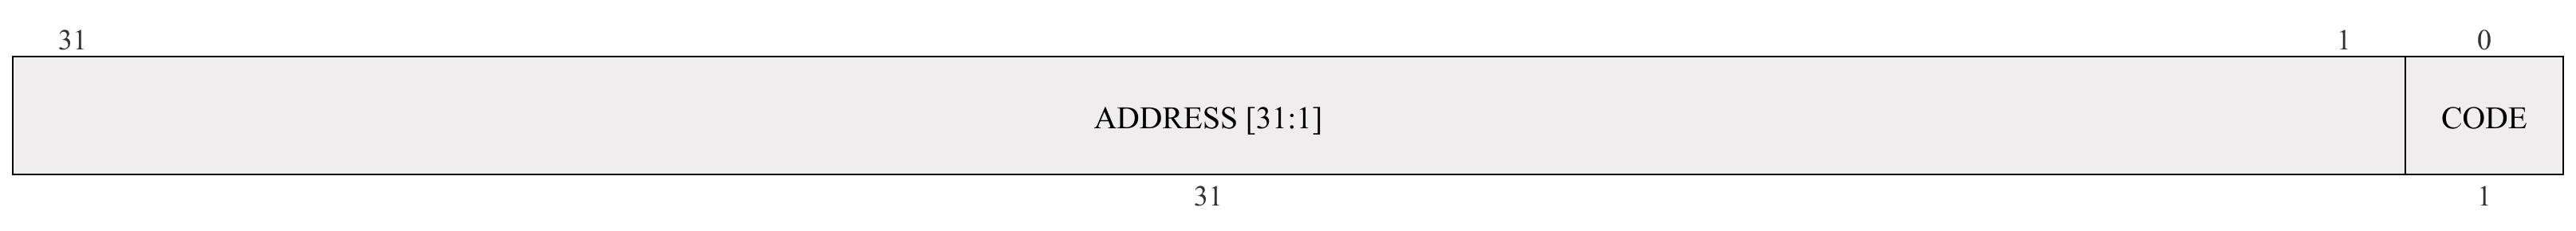
\includegraphics[width=.9\linewidth]{images/ecall_code.png}
  \caption{Encoding of register a7 during ecall}
  \label{fig:ecall}
\end{figure}

Forward edge controls are performed thanks to the Control Flow Graph and are further
explained in section \ref{sec:project_cfg} while backward edge controls are performed
thanks to the Shadow Stack and are further explained in section \ref{sec:project_ss}.

\section{Shadow Stack}
\label{sec:project_ss}

The file \textit{shadow\_stack.c} holds the configuration for the Shadow Stack.
The development of the Shadow Stack took inspiration from the formally verified
idea proposed by Matthieu Baty, Guillaume Hiet, and Pierre Wilke in their
article \textit{Work in progress: A formally verified shadow stack for RISC-V} \cite{shadowstack}.

The Shadow Stack is implemented as a standard Last-in-first-out stack (LIFO).
This is because the last jump that is performed in a code will always be the
first to return. This allowed us to build an effective and fast data structure that
consumes a small amount of memory.

The Shadow Stack allows two operations, \textit{push} and \textit{pop}. \textit{Push}
is used when a direct or indirect jump is made. If such a jump is considered legal,
its return address is pushed into the Shadow Stack and stored for later. Instead,
\textit{pop}, is used when a return is made. An address is \textit{popped} from
the Shadow Stack and a match between the popped value and the current return
address is made to decide whether the return instruction is legal or not.

\section{Control Flow Graph (CFG)}
\label{sec:project_cfg}

The Control Flow Graph of the binary is extracted during the instrumentation phase.
As we have seen, if there are indirect jumps the script performs a simulation run
to retrieve source and destination addresses of each indirect jump. If there is
a simulation, the output is parsed to store the addresses in a list. After that,
the static extraction begins, in which we examine the dump file of the binary to
retrieve the source and destination addresses of each direct call. After all the
addresses have been gathered, the lists are ordered and injected in the file
\textit{cfg.c} which holds the configuration for the Control Flow Graph.

In this file, we can see the structure of the Control Flow Graph which is an
array where each position is occupied by a pair \textit{source-destination}.
Since the CFG will not change during execution we can define it statically and
provide no functions to add or remove elements. The only available function is \textit{check}
which asks for a pair of addresses as input and determines whether such a pair
is part of the CFG or not. The check is implemented using a binary search function
and the comparison is made using the function depicted in Figure \ref{fig:binsearch}.
With this function, the binary search first searches for the source address and,
only when found it searches for the destination address.

This implementation of the Control Flow Graph effectively reduces space
consumption to the bare minimum while providing a fast checking method ($\mathcal{O}
(\log{n})$). Another solution could be to use a Hash Table to store the addresses.
In this case, we would reduce the time required to access the CFG to $\mathcal{O}
(1)$. However, this works only with big enough Hash Tables, otherwise, we could face
many collisions, and the time required to find the correct entry would increase.
Still, this alternative solution could be perfect for situations in which we
care more about time than space.

\begin{figure}[htbp]
  \centering
  \begin{lstlisting}[style=CStyle]
int compare(const int* A, const int* B) {
  for (int i = 0; i < 2; ++i) {
    if (A[i] < B[i]) return -1;
    if (A[i] > B[i]) return 1;
  }
  return 0;
}
 \end{lstlisting}
  \caption{Comparison for binary search}
  \label{fig:binsearch}
\end{figure}

\section{Physical Memory Protection (PMP)}
\label{sec:project_pmp}

In this project, the role of the PMP is to protect the Shadow Stack and the Control
Flow Graph from unauthorized modifications. To ensure that both these data
structures are secured four memory regions have been created. Each region's configuration
can be seen in Table \ref{tab:pmpregions}

\begin{table}
  \centering
  \begin{tabular}{|c|c|c|c|}
    \hline
    \textbf{Region Start}           & \textbf{Region End}           & \textbf{Type} & \textbf{Privileges} \\
    \hline
    0x00000000                      & End of .sdata region          & TOR           & R-W                 \\
    \hline
    Start of interrupt vector table & End of interrupt vector table & TOR           & R-W-X               \\
    \hline
    Start of Shadow Stack           & End of Control Flow Graph     & TOR           & R-W                 \\
    \hline
    Start of main                   & 0x90000000                    & TOR           & R-W-X               \\
    \hline
  \end{tabular}
  \caption{PMP memory regions}
  \label{tab:pmpregions}
\end{table}

The first region covers all the space between 0x00000000 and the end of the .sdata
region with read and write privileges, since this region contains only static data
there is no need to allow execution.

The second region covers the interrupt vector table and its functions, since
this region is accessed only in Machine mode and we need to execute instructions
we need to provide read, write, and instruction execution privileges.

The third region is the one that covers both the Shadow Stack and the Control
Flow Graph. For this reason, we need to restrict privileges to read and write. We
can't set this region as read-only since we need to modify the Shadow Stack during
execution.

The last region covers all the addresses from the start of the main function up to
the end of the memory. This region also includes user code and, since we need to
execute the code, we need to configure this region with read, write, and
instruction execution privileges.

This PMP configuration effectively helps to prevent unauthorized modifications
to critical components such as the Shadow Stack and the Control Flow Graph. Thanks
to this, we are sure that whatever value we read from these data structures will
be safe and trustable.

\section{Forward and Backward Edge Controls}
\label{sec:project_controls}

The most critical part of this project is about validating jump and return instructions
and this is done inside the interrupt vector table.

Forward edge controls are made thanks to the Control Flow Graph while backward edge
controls are made thanks to the Shadow Stack.

In this section, each control will be carefully explained to show how they work
and why they provide a certain degree of security.

\subsection{Forward Edge Controls}
\label{subsec:forward}

To perform a forward edge control we need three things. The first is the source
address, the second is the destination address, and the third is an oracle that
tells us if the pair source-destination is valid. As already explained the destination
address is retrieved from \textit{a7} which is passed as the ecall code. The source
register instead can be retrieved from mepc \ref{subsec:mepc}. As we have seen, when
a trap is taken mepc holds the address of the instruction that was interrupted.
Since the ecall generates the trap we can just add $4$ (size of the ecall) to
the address stored in mepc to retrieve the source address. Now that we have the pair
of addresses to check we can use the Control Flow Graph as the oracle. As
already explained, the CFG is computed before compilation and is securely stored
in a safe memory region so we can consider it as a trusted oracle.

So, when we need to perform a forward edge control, we can just send the source and
destination addresses to the \textit{check} function of the CFG. Such function performs
a binary search inside the CFG to see whether that specific pair is part of the original
CFG. If the search succeeds the function returns a positive value and the jump
is considered legal while, if the search does not succeed the instruction is aborted
and the execution terminates to prevent any possible damage.

Whenever a forward edge control succeeds we know that the related jump instruction
will eventually return so we need to store its return address inside the Shadow Stack.
To do so, we need to retrieve the return address but, since a call will always
return to its next instruction, we can just compute $source \ address + 2$ (size
of \textit{jal} and \textit{jalr}) to retrieve it. After that, the address is pushed
into the Shadow Stack, and the execution is resumed with the interrupted jump
instruction.

\subsection{Backward Edge Controls}
\label{subsec:backward}

To perform a backward edge control we need two things. The first is the
destination address and the second is an oracle that tells us if such address is
valid. As we have seen, the destination address is retrieved from \textit{a7} which
is passed as the ecall code. In this case, the oracle is the Shadow Stack.

So, when we need to perform a backward edge control, we can just pop an address from
the Shadow Stack and match the destination address with the popped one. If the
addresses are the same we consider the return instruction legal while, if they are
different the execution is terminated.

Whenever a backward edge control succeeds we must do nothing since the value has
already been removed from the Shadow Stack and no other modifications are needed.
Thus, the execution is resumed with the interrupted return instruction.

\section{Proof of Concept (PoC)}
\label{sec:project_poc}

In this section, we will see why the proposed solution effectively provides security
capabilities to a non-trusted and insecure code. Figure \ref{fig:functioning}
depicts an abstraction of the project's flow.

\begin{figure}[htbp]
  \centering
  \def\stackalignment{r}\stackunder{ 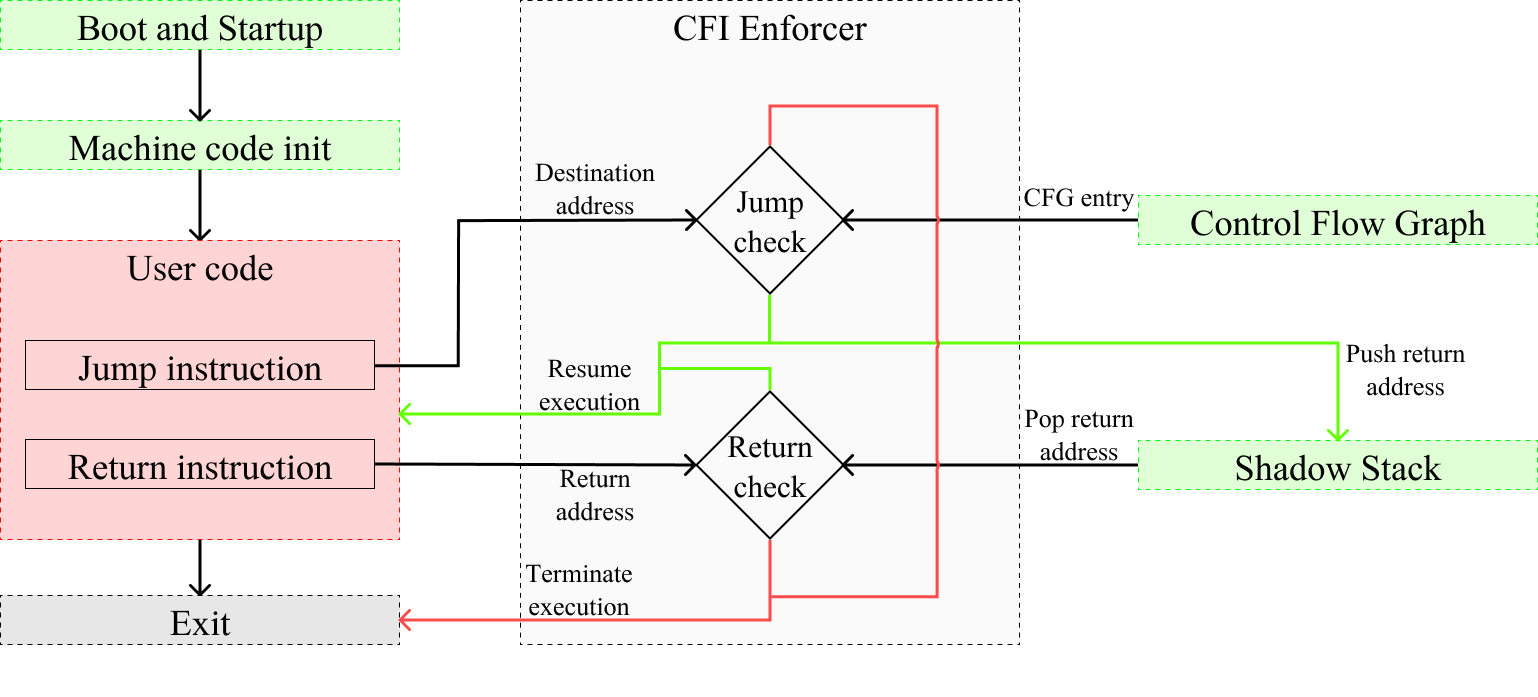
\includegraphics[width=.9\linewidth]{images/functioning.png} } %
  {\scriptsize }
  \caption{Abstraction of the flow of execution}
  \label{fig:functioning}
\end{figure}

We have already seen that the \textit{Boot and Startup} and \textit{Machine code
init} sections are used to configure the board and the machine configuration respectively.
This part of the code is trusted so we are sure the machine will be configured
properly. The only way to corrupt this part of the execution would be to modify the
source code before compilation but, this is out of the project's scope.

The same is true for the \textit{CFI Enforcer} section which is responsible for managing
edge controls as well as other interrupts and exceptions. Even in this case, the
source code has to be modified to tamper with the security features.

On the other hand, the \textit{User code} section is untrusted and we can't make
any assumptions on its functioning. The code could be well-written and somewhat
secure but it could be full of flaws and we must prevent any attack that could
be perpetrated through it. To do so, we use forward and backward edge controls
together with the Shadow Stack and the Control Flow Graph.

As already said, the Shadow Stack and the CFG are the most critical points of the
project. We must secure them since they serve as oracles and we must be able to
trust the data they contain. Since the CFG is configured statically we are sure that
it can't be modified during execution, the Shadow Stack instead is designed to
change since we need to push and pop values from it. However, since we protected
the Shadow Stack with the PMP we can be sure that only privileged code has
access to it and any other access generates a trap that is handled through the
interrupt vector table. This means that, even if one tries to add or remove
values from the stack the operation will be aborted immediately and our trust in
the Shadow Stack remains intact.

Now we will go through every possible scenario that could happen during a normal
execution.

As soon as a forward edge control is requested we check that the pair source-destination
is valid thanks to the CFG. Let's say that an attacker tampered with the code to
perform an unauthorized jump, in this case, the CFG will not contain such a pair
since we said that it can't be modified. In this case, the unauthorized jump is detected
and the code terminates immediately. Instead, if the pair is legal according to the
CFG the jump is considered safe and the return address is pushed into the Shadow
Stack. Note that since we compute the return address each time instead of
trusting the one provided by the user code we are sure that the value inserted
in the stack is correct and we can trust it.

If a backward edge control is requested instead, we check that the return address
provided by the user code is the one we are expecting by popping the last value that
was inserted in the Shadow Stack. Again, let's say that an attacker tampered with
the code to perform an unauthorized return, in this case, the addresses will not
match and the execution is terminated. Note that the fact that we can trust the
Shadow Stack is highly dependent on the configuration of the PMP. This is because,
without a proper configuration, it would be possible for an attacker to push a value
into the Shadow Stack and then tamper with the return address to effectively return
to an unauthorized address.

Moreover, when we try to push a value into a full Shadow Stack the execution is
terminated. This is needed because if we are not able to push the address into the
Shadow Stack we will not be able to make the next backward edge control and thus,
the security would be compromised. Note that the same happens when we try to pop
a value from an empty Shadow Stack since this means that we are checking a return
instruction that was never meant to be performed.

Lastly, we could design the enforcement of the backward edge controls in another
way. If we need to control a return address and there is a mismatch we could force
the user code to return to the address stored in the Shadow Stack which we know is
safe. While this solution enforces Control Flow Integrity securely we can't be
sure that the stack (referring to the normal stack used to store registers) has
not been compromised and thus, terminating execution is a much safer choice.

So, we have seen that this project effectively enforces Control Flow Integrity
on an untrusted user application and that its security functionalities work as
expected to prevent any attempt to perform unauthorized operations.

  \chapter{Threat Analysis}
\label{cha:ta}

\lipsum[1]

\section{Threat Model}
\label{sec:ta_model}

\lipsum[1]

\section{Testing Methodologies}
\label{sec:ta_methodologies}

\lipsum[1]

\section{Results and Analysis}
\label{sec:ta_analysis}

\lipsum[1]

\section{Limitations}
\label{sec:ta_limitations}

\lipsum[1]
  \chapter{Performance Analysis}
\label{cha:pa}

The purpose of this chapter is to examine and discuss \textit{STEERED}'s performance
impact on the code. Firstly, we present the difference in execution time between
a standard binary and a \textit{STEERED}-secured one. In this part we will give great
importance to the time overhead, describing the reason behind the collected
values. Secondly, we present the difference in size between the produced
binaries, giving great importance to memory overhead. Lastly, we provide an analysis
of the obtained results as well as some optimization ideas to further reduce the
performance impact of \textit{STEERED} on the code.

The performance analysis took inspiration from the articles \textit{Efficient
CFI Enforcement for Embedded Systems Using ARM TrustZone-M}\cite{article1} (Gisu
Yeo, Yeryeong Kim et al., 2022) and \textit{PROLEPSIS: Binary Analysis and Instrumentation
of IoT Software for Control-Flow Integrity}\cite{article2} (Valentina Forte, Nicol\`{o}
Maunero et al., 2021) where the writers propose a solution similar to \textit{STEERED}
for \textit{ARM}-based embedded devices. We tested the infrastructure on the same
algorithms proposed by the papers, providing tests on $13$ different algorithms
+ $4$ variations with indirect jumps.

Moreover, to present correct and realistic data, all tests have been conducted
on the aforementioned \textit{Espressif's ESP32-C3-DevKitM-1}.

\section{Time Performances}
\label{sec:pa_time}

In this section, we will see how \textit{STEERED}'s infrastructure affects the
execution time of the code. Two histograms depicting test results can be seen in
Figures \ref{fig:lowtime} and \ref{fig:hightime}, note that execution times have
been separated into two different charts to enhance readability.

\begin{figure}[htbp]
  \centering
  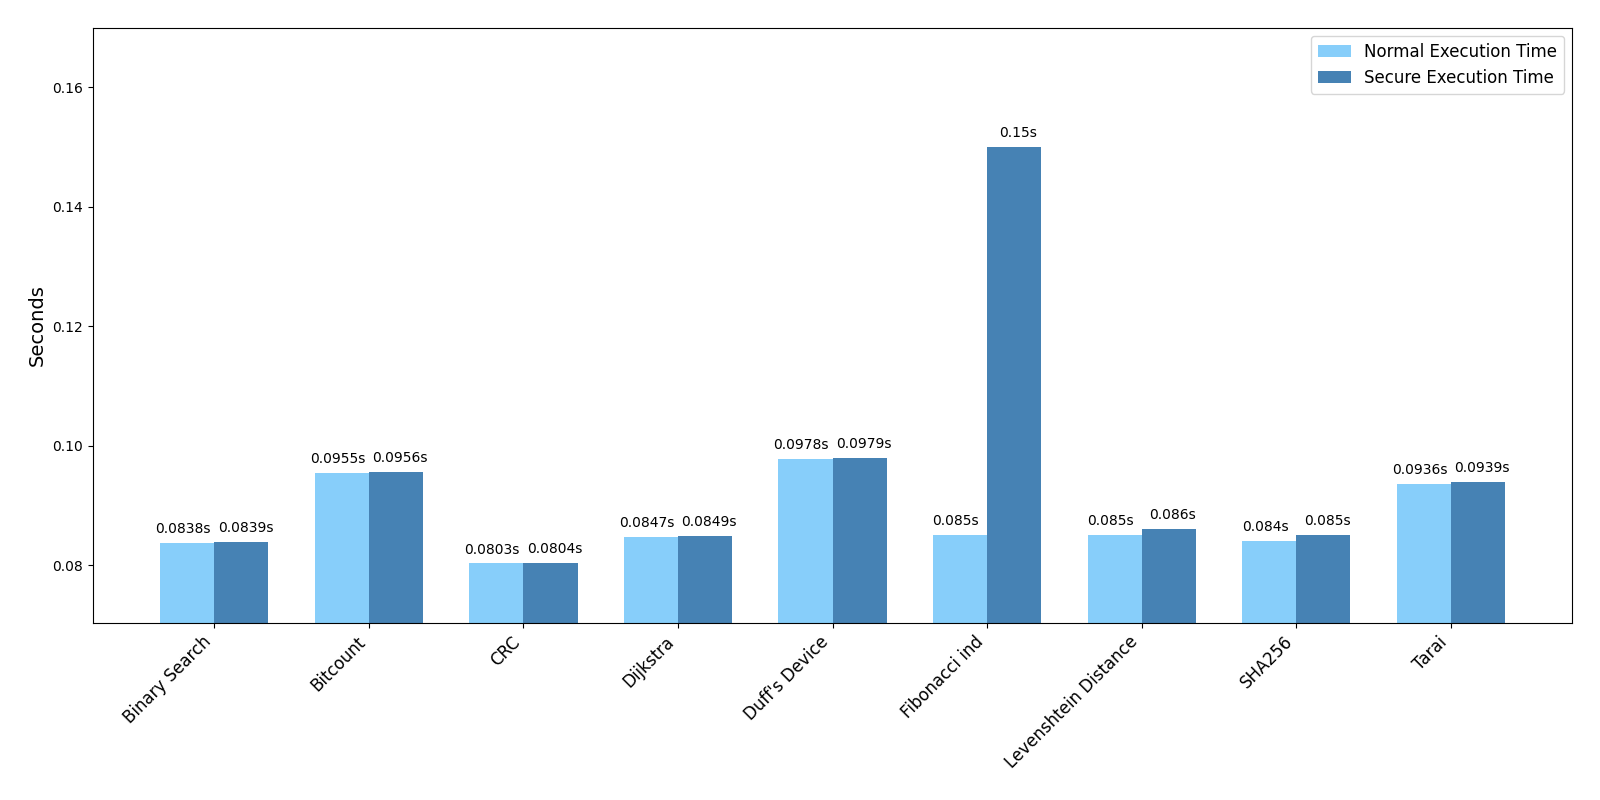
\includegraphics[width=\linewidth]{images/low_times.png}
  \caption{Comparison between binaries execution times (low times)}
  \label{fig:lowtime}
\end{figure}

\begin{figure}[htbp]
  \centering
  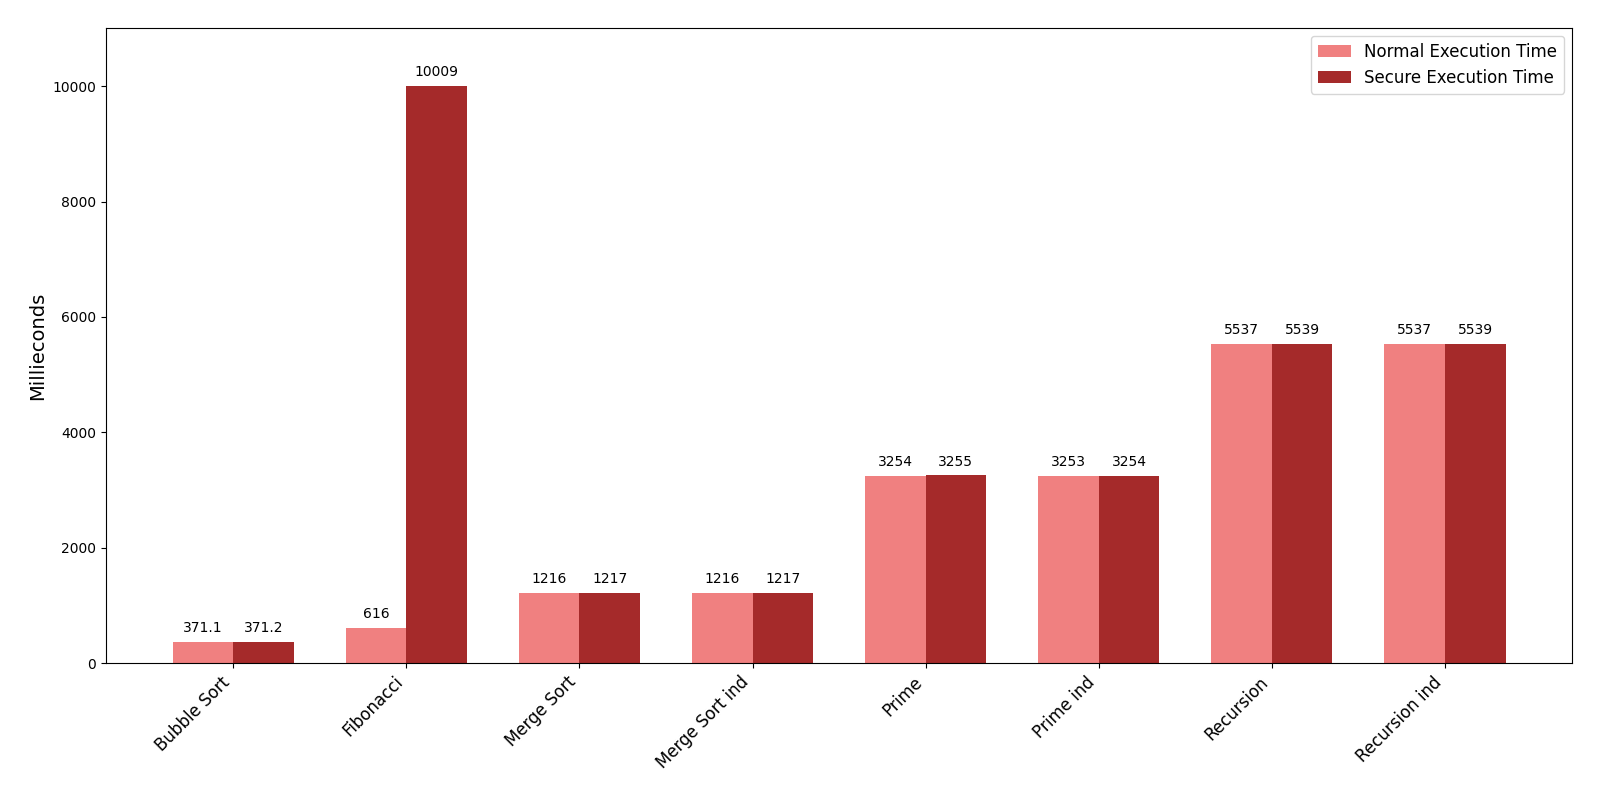
\includegraphics[width=\linewidth]{images/high_times.png}
  \caption{Comparison between binaries execution times (medium and high times)}
  \label{fig:hightime}
\end{figure}

Table \ref{tab:times} depicts test results for each algorithm as well as the
percentage of time overhead. As we can see, in most cases the time overhead
affects the fourth or fifth digit resulting in an unnoticeable increase in
execution time. However, there are two cases in which the time overhead is very
big and it impacts performances in a relevant way.

\begin{table}
  \centering
  \begin{tabular}{|c|c|c|c|}
    \hline
    \textbf{Algorithm}                   & \textbf{Normal run time (s)} & \textbf{Secure run time (s)} & \textbf{Time Overhead} \\
    \hhline{====} \textit{Binary Search} & 0.08387                      & 0.08388                      & $0.012\%$              \\
    \hline
    \textit{Bitcount}                    & 0.0955                       & 0.0956                       & $0.11\%$               \\
    \hline
    \textit{Bubble Sort}                 & 0.37113                      & 0.37116                      & $0.008\%$              \\
    \hline
    \textit{CRC}                         & 0.08025                      & 0.08026                      & $0.012\%$              \\
    \hline
    \textit{Dijkstra}                    & 0.0847                       & 0.0849                       & $0.236\%$              \\
    \hline
    \textit{Duff's Device}               & 0.097795                     & 0.097799                     & $0.0041\%$             \\
    \hline
    \textit{Fibonacci}                   & 0.6166                       & 10.0089                      & $1523.24\%$            \\
    \hline
    \textit{Fibonacci Indirect}          & 0.0849                       & 0.1511                       & $77.97\%$              \\
    \hline
    \textit{Levenshtein Distance}        & 0.085                        & 0.086                        & $1.176\%$              \\
    \hline
    \textit{Merge Sort}                  & 1.216                        & 1.217                        & $0.0822\%$             \\
    \hline
    \textit{Merge Sort Indirect}         & 1.2168                       & 1.2169                       & $0.0082\%$             \\
    \hline
    \textit{Prime}                       & 3.254                        & 3.255                        & $0.03\%$               \\
    \hline
    \textit{Prime Indirect}              & 3.253                        & 3.254                        & $0.03\%$               \\
    \hline
    \textit{Recursion}                   & 5.537                        & 5.539                        & $0.036\%$              \\
    \hline
    \textit{Recursion Indirect}          & 5.537                        & 5.539                        & $0.036\%$              \\
    \hline
    \textit{SHA256}                      & 0.084                        & 0.085                        & $1.19\%$               \\
    \hline
    \textit{Tarai}                       & 0.0936                       & 0.0939                       & $0.32\%$               \\
    \hline
  \end{tabular}
  \caption{Test results for execution times}
  \label{tab:times}
\end{table}

It is straightforward to understand why the overhead is small for algorithms like
\textit{Binary Search} and \textit{Duff's Device} since these programs perform few
jumps and most of the computation is performed inside a while or for loop so,
the overhead given by the instrumentation is unnoticeable if compared to the
total execution time. For example, the \textit{Binary Search} algorithm performs
$3$ jump instruction and $3$ return instructions even if it is working on a rather
big array. Given this behavior, such a small time overhead is expected in similar
situations.

Instead, examples like \textit{Prime} and \textit{Recursive} are a bit trickier.
Since these algorithms work with a recursive approach they perform many control transfer
instructions consequently thus, we expect the time required for the context
switch and the forward and backward edge controls to be somewhat impactful. However,
results show that even in these cases the difference is barely noticeable\footnote{In
these cases instead of impacting the fourth or fifth digit the overhead impacts
the second or third digit.}. The reason could be due to the processor's
frequency which, in the case of \textit{Espressif's ESP32-C3-DevKitM-1}, is $160
\ MHz$. This means that the CPU is able to execute the secure and non-secure
binaries in similar times. For example, the \textit{Recursion} algorithm performs
$\sim 4000$ jump instructions and $\sim 4000$ return instructions which translates
to $\sim 8000$ edge controls and $\sim 16000$ context switches\footnote{The
number is doubled because for each edge control we need to increase the
privilege to M-mode, perform the control, and then return to U-mode, resulting in
two context switches.}. However, if we compare those numbers to the $160$
million operations the processor can perform in a second we see why the time
overhead is so small. Note that we add $2$ instructions for every jump instruction
and $3$ instructions for every return instruction, resulting in an instruction
overhead of $4000*2 + 4000*3 = 20000$. Moreover, the handling of forward and
backward edge controls requires $\sim 800$ instructions which results in
$(4000 + 4000) * 800 = 6400000$ total instructions. Now, if we compute
$\frac{20000 + 6400000}{160000000}$ we discover that the utilized processor can
perform all these instructions in $\sim 0.04$ seconds. Depending on the algorithm
and the recursion depth we see that the overhead is affecting the second or third
digit.

Two peculiar cases are the ones of the \textit{Fibonacci} and \textit{Fibonacci
Indirect} algorithms, in these cases, the overheads are $1523.24\%$ and $77.97\%$
respectively. The possible reason for these enormous overheads is that these
algorithms make two recursive calls each time so we end up with an exponential
amount of jump and return instructions. This leads to many edge controls and the
execution is strongly affected by this.

Overall, \textit{STEERED} achieved an average time overhead of $94.38\%$ with a standard
deviation of $368.68$. However, if we do not take into account the outliers we can
see that the median is $0.036\%$. These results clearly show that \textit{STEERED}'s
time overhead is almost unnoticeable in many cases but, this also demonstrates
that the project strongly suffers from deeply recursive algorithms and that
further optimization is required to reduce the time impact on these types of
algorithms.

Lastly, in Table \ref{tab:othertimes} we provide the times required to instrument
the code, extract the CFG, and perform the simulation. As we can see the
instrumentation and CFG extraction phases always require less than a fraction of
a second to finish. However, we must take into consideration that the tested
algorithms are composed of few lines of code and the situation could change if
we were to instrument a firmware composed of thousands of lines. The simulation instead
requires a lot of time, even algorithms that run in a second or less require a
few seconds to simulate. This is due to the logging required to extract the indirect
jump destinations which affects the time performances seriously. Note that we
can accept this result since the simulation is run only once and the logging is
removed from the final binary so that this overhead does not affect the actual
execution.

\begin{table}
  \centering
  \begin{tabular}{|c|c|c|c|}
    \hline
    \textbf{Algorithm}                   & \textbf{Instrumentation (s)} & \textbf{Simulation (s)} & \textbf{CFG extraction (s)} \\
    \hhline{====} \textit{Binary Search} & 0.00296                      & no ind jumps            & 0.00174                     \\
    \hline
    \textit{Bitcount}                    & 0.00196                      & no ind jumps            & 0.00153                     \\
    \hline
    \textit{Bubble Sort}                 & 0.00302                      & no ind jumps            & 0.00175                     \\
    \hline
    \textit{CRC}                         & 0.00203                      & no ind jumps            & 0.00154                     \\
    \hline
    \textit{Dijkstra}                    & 0.00264                      & no ind jumps            & 0.00182                     \\
    \hline
    \textit{Duff's Device}               & 0.00265                      & no ind jumps            & 0.00163                     \\
    \hline
    \textit{Fibonacci}                   & 0.00209                      & no ind jumps            & 0.00149                     \\
    \hline
    \textit{Fibonacci Indirect}          & 0.00202                      & 130.5567                & 0.07037                     \\
    \hline
    \textit{Levenshtein Distance}        & 0.00255                      & no ind jumps            & 0.00167                     \\
    \hline
    \textit{Merge Sort}                  & 0.00354                      & no ind jumps            & 0.00178                     \\
    \hline
    \textit{Merge Sort Indirect}         & 0.0036                       & 4.6394                  & 0.00273                     \\
    \hline
    \textit{Prime}                       & 0.00214                      & no ind jumps            & 0.00168                     \\
    \hline
    \textit{Prime Indirect}              & 0.00208                      & 11.4051                 & 0.00451                     \\
    \hline
    \textit{Recursion}                   & 0.00202                      & no ind jumps            & 0.00159                     \\
    \hline
    \textit{Recursion Indirect}          & 0.00202                      & 23.2751                 & 0.00875                     \\
    \hline
    \textit{SHA256}                      & 0.00411                      & no ind jumps            & 0.00189                     \\
    \hline
    \textit{Tarai}                       & 0.00198                      & no ind jumps            & 0.00152                     \\
    \hline
  \end{tabular}
  \caption{Test result for instrumentation phases}
  \label{tab:othertimes}
\end{table}

\section{Memory Overhead}
\label{sec:pa_memory}

In this section, we showcase how \textit{STEERED}'s infrastructure affects the
size of the produced binary. A histogram depicting test results can be seen in Figure
\ref{fig:binsize}.

\begin{figure}[htbp]
  \centering
  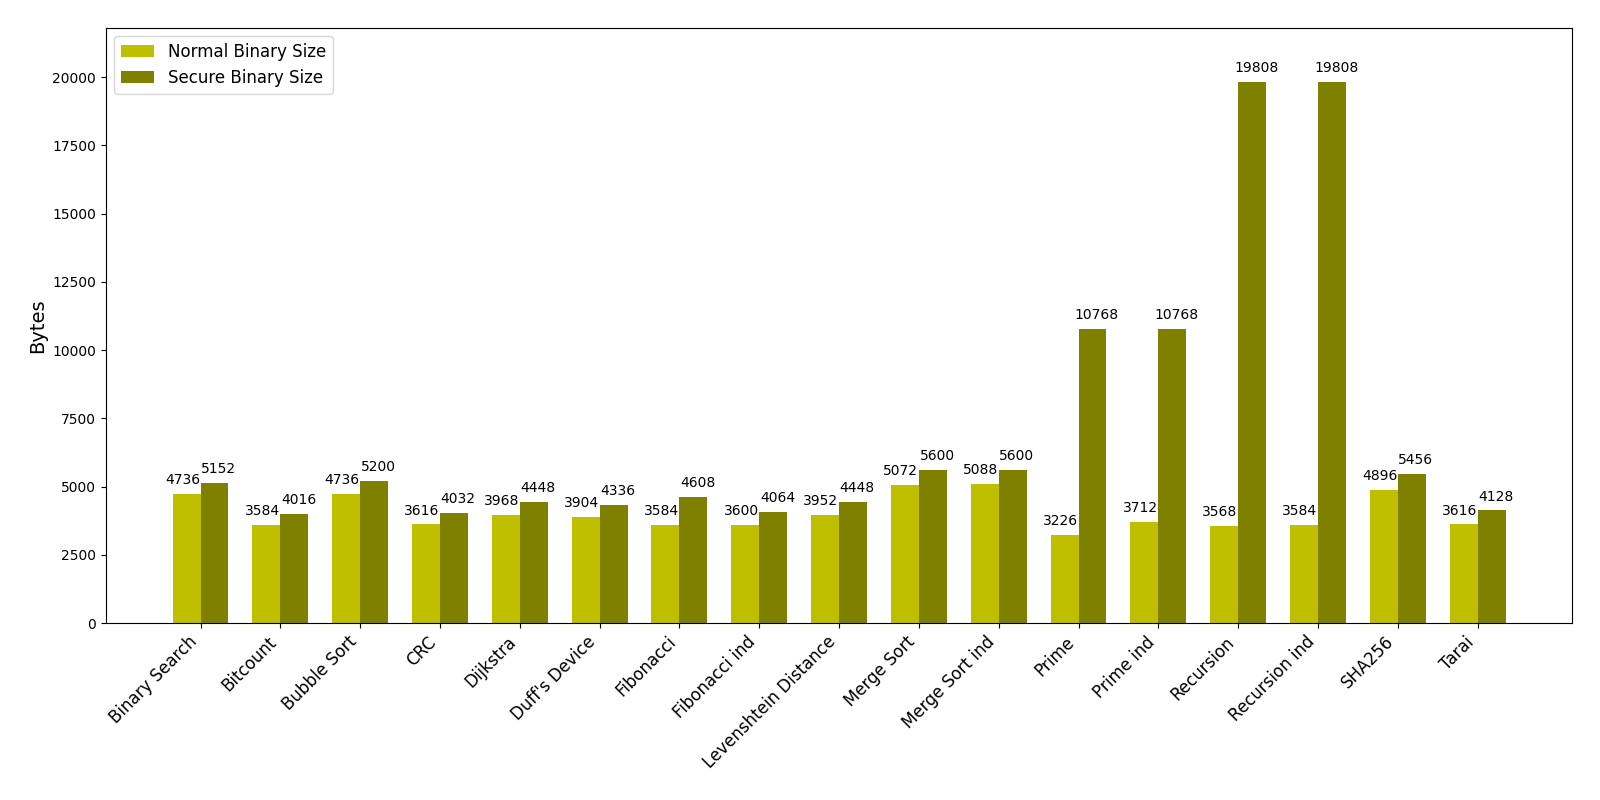
\includegraphics[width=\linewidth]{images/size.png}
  \caption{Comparison between binaries size}
  \label{fig:binsize}
\end{figure}

Table \ref{tab:binsize} depicts test results for each algorithm as well as the
percentage of memory overhead. As we can see, in most cases the size of the
binary increases by $\sim 10\%$. This is due to the Shadow Stack, Control Flow
Graph, and the instructions added during instrumentation.

As for the time analysis, there are some peculiar cases. \textit{Prime}, \textit{Recursion}
and their indirect variations \textit{Prime Indirect} and \textit{Recursion
Indirect}, present an overhead of $\sim 200\%$ and $\sim 450\%$ respectively.
This happens because these recursive algorithms perform all the jump
instructions consecutively and then all the return instructions. This means that
we must allocate a Shadow Stack big enough to store all the return addresses to ensure
correct backward edge controls. For example, we have seen that the \textit{Recursion}
algorithm performs $\sim 4000$ jump instructions, this means that we must create
a Shadow Stack that can store at least $4000$ addresses. Given that an address
is stored as an \textit{unsigned int}, we can easily see that a Shadow Stack
that can store $4000$ addresses occupies $4000*4 = 16000 \ \textit{Bytes}$\footnote{We
multiply by $4$ because it is the size of an \textit{unsigned int} in C.}. Now, if
we take the size of the secure binary for the \textit{Recursion} algorithm we
can calculate $19808 - 16000 = 380 8 \ \textit{Bytes}$, so, apart from the
Shadow Stack, the binary has an overhead of $\frac{3808-3568}{3568}*100 = \sim 6.
73\%$ which is similar to the other ones.

Note that this problem is related strictly to recursive algorithms as they perform
a high number of jumps and then they start performing the first return instruction.
However, we could have a similar problem with the Control Flow Graph as for a big
binary like a firmware we can have many different jump instructions, and, as a consequence,
the CFG would drastically increase in size.

\begin{table}
  \centering
  \begin{tabular}{|c|c|c|c|}
    \hline
    \textbf{Algorithm}                   & \textbf{Normal bin size (B)} & \textbf{Secure bin size (B)} & \textbf{Memory Overhead} \\
    \hhline{====} \textit{Binary Search} & 4736                         & 5152                         & $8.78\%$                 \\
    \hline
    \textit{Bitcount}                    & 3584                         & 4016                         & $12.05\%$                \\
    \hline
    \textit{Bubble Sort}                 & 4736                         & 5200                         & $9.79\%$                 \\
    \hline
    \textit{CRC}                         & 3616                         & 4032                         & $11.51\%$                \\
    \hline
    \textit{Dijkstra}                    & 3968                         & 4448                         & $12.09\%$                \\
    \hline
    \textit{Duff's Device}               & 3904                         & 4336                         & $11.06\%$                \\
    \hline
    \textit{Fibonacci}                   & 3584                         & 4608                         & $28.57\%$                \\
    \hline
    \textit{Fibonacci Indirect}          & 3600                         & 4064                         & $12.88\%$                \\
    \hline
    \textit{Levenshtein Distance}        & 3952                         & 4448                         & $12.55\%$                \\
    \hline
    \textit{Merge Sort}                  & 5072                         & 5600                         & $10.41\%$                \\
    \hline
    \textit{Merge Sort Indirect}         & 5088                         & 5600                         & $10.06\%$                \\
    \hline
    \textit{Prime}                       & 3226                         & 10768                        & $233.78\%$               \\
    \hline
    \textit{Prime Indirect}              & 3712                         & 10768                        & $190.08\%$               \\
    \hline
    \textit{Recursion}                   & 3568                         & 19808                        & $455.15\%$               \\
    \hline
    \textit{Recursion Indirect}          & 3584                         & 19808                        & $452.68\%$               \\
    \hline
    \textit{SHA256}                      & 4896                         & 5456                         & $11.43\%$                \\
    \hline
    \textit{Tarai}                       & 3616                         & 4128                         & $14.16\%$                \\
    \hline
  \end{tabular}
  \caption{Test results for memory consumption}
  \label{tab:binsize}
\end{table}

Overall, \textit{STEERED} achieved an average memory overhead of $88.06\%$ with a
standard deviation of $152.77$. However, similarly to the time overhead, if we
do not take into consideration the outliers we can see that the median is
$1 2.09 \%$. These results show that in most cases \textit{STEERED} can produce
a secure binary without affecting too much memory consumption. Even in this case,
the project suffers from deeply recursive algorithms as we need to allocate a
bigger Shadow Stack to securely store each address.

\section{Results and Analysis}
\label{sec:pa_results}

In this section, we discuss the obtained result and showcase the weak points of
\textit{STEERED}.

As we have seen in the previous sections the project showcases promising performances
in most cases. In almost all the tested algorithms time overhead was barely
noticeable and memory consumption was acceptable. Overall, the project
infrastructure is not impacting the normal performances of the non-secure binary.

However, in the case of deeply recursive algorithms, we have seen that the time
overhead grows exponentially due to the high number of control transfer
instructions and the related forward and backward edge controls. Also, the size
of the binary grows as we need a bigger Shadow Stack to store all the addresses
needed to perform the backward edge controls.

Moreover, we have seen that if the code is composed of thousands of lines it is likely
that the Control Flow Graph will be very big. This is because if we have many
jump instructions from different sources to different destinations we must store
each pair, thus the space occupied by the CFG grows.

In the following section, we provide some optimization techniques that could be
applied to further increase \textit{STEERED}'s performances. Specifically, we provide
alternative solutions to improve the weak points of the project.

\section{Optimization Techniques}
\label{sec:pa_optimization}

Since optimization is a key factor when developing projects on embedded devices
given their hardware limitations we tried to provide an infrastructure as fast
as possible while preserving memory usage. However, as test results show, there are
some aspects of the project that require further improvement to be considered acceptable.

The two identified cases in which \textit{STEERED} strongly impacts the
performances are:
\begin{itemize}
  \item Deeply recursive algorithms: we have seen that deeply recursive
    algorithms require a big Shadow Stack to hold all the return addresses and
    thus, they require a lot of extra memory. To solve this issue we could
    modify the Shadow Stack in the following way. When we see that a function calls
    itself many times we could store the return address only one time and introduce
    a \textit{peek} function. With this, we could still perform the backward
    edge controls when we need to but we would need to store the address only
    once. Then, if we need to perform a control on another address we would just
    need to \textit{pop} the ``recursive'' address and then \textit{pop} the
    following one to see if it matches with the one we are checking. With such modification,
    we could effectively reduce the amount of space occupied by the Shadow Stack
    in case of recursive algorithms without impacting the security features that
    \textit{STEERED} provides;

  \item Big user code: we have seen that with very big codes (like the aforementioned
    firmware one) we could end up in a situation where the Control Flow Graph
    grows bigger and bigger due to the high amount of control transfer
    instructions from different sources to different destinations. Unfortunately,
    we can do nothing about memory consumption in this case as we can't afford
    to avoid storing some source-destination pairs. However, as already
    explained we could implement a Hash Table which would not decrease the
    memory consumption but, at least we could reduce the time required to access
    the Control Flow Graph from $\mathcal{O}(\log{n})$ to $\mathcal{O}(1)$.
\end{itemize}

Lastly, we provide a space optimization solution that could be implemented for very
small source code. Say, for example, that the \textit{.text} section that we want
to instrument starts at address $0x4038A000$ and ends at address $0x4038A000$.
Since the first part of the address stays the same it provides no useful
information, thus we could apply a bit-mask to remove $4038$ from the address,
storing only the last $16$ bits. This means that we would be able to store an address
inside an \textit{unsigned short} instead of an \textit{unsigned int}. As a
result, we would be able to halve the space required to store the Control Flow Graph
and the Shadow Stack resulting in a great improvement in memory consumption.
However, this solution only works when the user code is very small because if the
\textit{.text} section starts at address $0x4038A000$ and ends at address
$0x4039F000$ we would still need an \textit{unsigned int} to store a correct representation
of the address.

In conclusion, our analysis has demonstrated that the \textit{STEERED} framework
exhibits commendable performance in a variety of scenarios. Nevertheless, there are
specific edge cases where its efficiency can be significantly compromised,
leading to suboptimal results. These instances reveal potential vulnerabilities in
the system that could hinder its overall effectiveness. To address these
challenges, we suggest implementing the proposed solutions, which aim to refine
the project's functionality. By fine-tuning the system to better adapt to particular
situations, we can effectively minimize both memory usage and processing time, thereby
enhancing the overall performance and reliability of \textit{STEERED}.
  \chapter{Real-Time OS and STEERED}
\label{cha:rtos}

\textit{STEERED} has been developed and tested on bare-metal applications to ensure
its correctness in simple environments. However, many embedded devices are designed
to accomplish more complex tasks and they need special environments to support the
execution. The purpose of this chapter is to provide insights on how \textit{STEERED}
could be implemented to work with Real-Time Operating Systems (RTOS) to secure and
support complex tasks and environments. Specifically, we provide an implementation
idea for two famous RTOSes, \textit{Free Real-Time Operating System} (\textit{FreeRTOS})
and \textit{Zephyr RTOS}, depicting their strength and the limitations that may
arise during implementation.

\section{FreeRTOS}
\label{sec:rtos_rtos}

\textit{FreeRTOS}\cite{freertos} is an open-source, lightweight, Real-Time Operating
System kernel designed for embedded systems. In recent years, \textit{FreeRTOS}
has become one of the most widely used \textit{RTOS} kernels in embedded applications,
particularly in microcontrollers, because of its simplicity, efficiency, scalability,
and portability. \textit{FreeRTOS} is mostly used in applications that require
reliable, deterministic behavior in resource-constrained environments such as medical
devices, IoT devices, and automotive systems.

\textit{FreeRTOS} provides many key features:
\begin{itemize}
  \item Real-Time Scheduling: \textit{FreeRTOS} supports real-time scheduling with
    both preemptive and cooperative multitasking. In preemptive scheduling, tasks
    are prioritized and can interrupt lower-priority tasks, while in cooperative
    multitasking, tasks yield control to others explicitly. Moreover, it uses priority-based
    scheduling, allowing developers to assign priority levels to tasks based on
    their timing requirements;

  \item Task Management: Tasks in \textit{FreeRTOS} are individual threads of execution,
    each with its stack and context. The kernel allows the creation, deletion, and
    management of tasks dynamically. Each task operates in its own context, which
    the kernel saves and restores during context switching;

  \item Memory Management: \textit{FreeRTOS} provides several memory allocation schemes,
    including static and dynamic allocation, through its portable memory allocation
    subsystem. It supports different heap management schemes (\textit{heap\_1}
    through \textit{heap\_5}), offering varying levels of complexity and memory usage
    optimization. These schemes allow developers to balance between simplicity
    and flexibility;

  \item Interrupt Handling: \textit{FreeRTOS} is designed to work seamlessly with
    hardware interrupts, allowing Interrupt Service Routines (ISR) to
    communicate with tasks through mechanisms like queues and semaphores. The kernel
    offers a low-latency method for ISR handling, enabling efficient
    communication between ISRs and tasks while ensuring minimal delay in task
    scheduling;

  \item Software Timers: \textit{FreeRTOS} includes a timer API, allowing
    developers to create software timers that automatically trigger callback
    functions after a specified period. This feature helps to manage time-dependent
    operations without creating dedicated tasks;

  \item Portability and Scalability: \textit{FreeRTOS} is highly portable and can
    be adapted to run on numerous processor architectures, including \textit{ARM
    Cortex-M}, \textit{ARM Cortex-A}, \textit{RISC-V}, and various other
    architectures. It is structured in a way that allows developers to scale applications
    easily by adding or removing tasks, memory management schemes, and communication
    mechanisms as needed;

  \item Debugging and Traceability: \textit{FreeRTOS} provides support for debugging
    and traceability, offering hooks that allow users to gather runtime
    statistics and monitor task execution patterns.
\end{itemize}

With all these features it is easy to see why \textit{FreeRTOS} has become a standard
in the community. However, \textit{FreeRTOS} presents some limitations like the
limited built-in security and the lack of support for multicore processing. Some
of these flaws have been addressed by community users and companies with alternative
versions of the Operating System. For example, \textit{Espressif} presented
\textit{IDF FreeRTOS}\cite{idfrtos}, a version of \textit{FreeRTOS} which
provides support for multicore processing. Moreover, \textit{highintegritysystems}
developed \textit{SAFERTOS}\cite{safertos}, a redesign of the \textit{FreeRTOS} kernel
to enhance security.

Overall, \textit{FreeRTOS} is a powerful choice for developers working with embedded
systems that require real-time capabilities, low overhead, and efficient resource
management. Its design balances simplicity with flexibility, making it suitable for
a wide variety of applications from small IoT devices to more complex industrial
systems.

\section{Zephyr RTOS}
\label{sec:rtos_zephyr}

\textit{Zephyr RTOS}\cite{zephyrtos} is an open-source, Real-Time Operating System
designed for embedded systems and IoT applications. Developed under the Linux
Foundation, it offers a lightweight, modular, and scalable platform that supports
a wide range of devices, from simple microcontrollers to complex systems. Widely
adopted across IoT devices, industrial automation, medical equipment, and
automotive systems, \textit{Zephyr RTOS} excels in environments requiring
reliability, efficiency, and resource optimization.

A key feature of \textit{Zephyr} is its scalability and modularity. Its
architecture enables developers to include only the features they need, optimizing
memory usage and performance for resource-constrained devices. The kernel
supports multiple configurations, making it adaptable for both simple single-threaded
tasks and advanced multi-threaded applications. Additionally, \textit{Zephyr} is
designed to deliver deterministic, time-critical performance, ensuring minimal
latency and high reliability.

\textit{Zephyr} includes advanced security features such as memory protection,
secure boot, and support for Hardware Security Modules (HSMs). Regular updates
and audits ensure compliance with stringent security standards, making it a robust
choice for applications demanding high reliability and safety.

While both \textit{Zephyr RTOS} and \textit{FreeRTOS} are widely used in embedded
systems, they differ in their architecture, feature set, and target use cases. Firstly,
\textit{Zephyr} provides a comprehensive ecosystem out of the box, including
networking stacks, device drivers, and file systems. \textit{FreeRTOS}, in contrast,
offers a minimal kernel focused on task scheduling and real-time performance, with
additional features like networking provided as optional libraries. Moreover, \textit{Zephyr}
supports more complex applications, including those requiring multi-threading and
multi-core systems, making it suitable for advanced IoT and industrial devices. \textit{FreeRTOS}
is lightweight and optimized for simple real-time tasks on resource-constrained
microcontrollers. Lastly, \textit{Zephyr} offers built-in security features while
\textit{FreeRTOS} provides basic security features and relies on external
libraries for advanced functionalities.

Overall, with its lightweight design, real-time capabilities, and extensive ecosystem,
\textit{Zephyr RTOS} is a versatile platform for developers building secure,
scalable, and efficient embedded solutions.

\section{FreeRTOS, Zephyr RTOS, and STEERED}
\label{sec:rtos_porting}

In this section, we provide a detailed description of how \textit{FreeRTOS}
could be implemented to work inside \textit{STEERED}and why this could increase
the scenarios in which \textit{STEERED} could be used. Note that we focus on the
implementation of \textit{FreeRTOS} but, most of the information provided in
this section can be applied to the implementation of \textit{Zephyr RTOS}. The
same is true for the limitations discussed in Section \ref{sec:rtos_limitations}
as they suffer from the same implementation problem.

We have seen that \textit{STEERED} is designed to securely run untrusted user code
in bare-metal environments. However, given its simplicity, it could be used to
secure code in more complex environments, for example with a Real-Time Operating
System like \textit{FreeRTOS}.

The main idea is to maintain \textit{STEERED} as the M-mode operator, managing
system boot and edge controls. The user code in this case is represented by the various
tasks generated thanks to \textit{FreeRTOS}. Code instrumentation would not change
much as we would just need to add the \textit{regex} functions to search for
\textit{FreeRTOS}-specific instructions that cause a control transfer during execution.
Finally, \textit{FreeRTOS} could be used as a ``supervisor'', either trusted or untrusted
depending on the case. It would be in charge of managing task scheduling and
memory operations.

Moreover, since \textit{FreeRTOS} requires its own Interrupt Service Routine we
could either:
\begin{itemize}
  \item Prepare two separate Interrupt Vector Tables, one for \textit{STEERED}\footnote{The
    same we have seen in Section \ref{sec:project_isr}} and one for \textit{FreeRTOS}.
    However, traps at the user level are managed by default ad machine level so,
    if we have an interrupt or an exception in one of the tasks the controls is
    transferred to the \textit{STEERED} interrupt vector table and we must manually
    transfer the flow to the correct handler of the \textit{FreeRTOS} interrupt
    vector table;

  \item Another solution could be to prepare two separate interrupt vector tables
    and use \textit{mideleg} and \textit{medeleg} registers (seen in Section
    \ref{subsec:riscv_deleg}) to automatically delegate some interrupts and/or exceptions
    to the \textit{FreeRTOS} interrupt vector table. For example, if we know
    that user interrupts are always managed by \textit{FreeRTOS} we could insert
    the corresponding code inside \textit{mideleg}. With this, each time a user-level
    interrupt is generated it is trapped at the \textit{FreeRTOS} interrupt vector
    table. Note that this does not mean that \textit{STEERED} will not be able to
    manage those traps as higher-level interrupts and exceptions can't be delegated
    to the lower-level handler. For example, if a machine-level interrupt is generated
    it will always be handled by \textit{STEERED} interrupt vector table;

  \item The last solution would be to use only \textit{STEERED}'s interrupt
    vector table specifying that \textit{FreeRTOS} should trap exception and interrupts
    at such table. This means that every time a trap is taken in \textit{FreeRTOS}
    the execution is transferred to \textit{STEERED}'s handlers. However, this
    may result in two unwanted situations. Firstly, handling all the traps
    inside \textit{STEERED}'s interrupt vector table may require many controls and
    the code may become overly verbose. Secondly, this means that the traps that
    are generated in \textit{FreeRTOS} are handled in machine mode, and, for
    some environments, this could constitute a problem if we want to keep separation
    between privileges.
\end{itemize}

\section{Porting Limitations}
\label{sec:rtos_limitations}

The proposed implementation presents one key limitation, \textit{FreeRTOS} needs
to perform some operations on Control and Status Registers to function correctly
but, as we have explained such registers are only available in machine mode. Since
the implementation inside \textit{STEERED} would require \textit{FreeRTOS} to run
either in supervisor or user mode all those operations would generate an illegal
instruction exception as those privilege modes can't access machine CSRs. The
operations are depicted in Listing \ref{lst:freeoperations}.

To address this problem we could enhance the instrumentation phase to modify
\textit{FreeRTOS}'s code in the following way. Firstly, we need to find the critical
instructions, this can be done easily with \textit{regex} functions. With this, we
can extract the operation that \textit{FreeRTOS} is trying to perform (among the
one seen in Section \ref{sec:riscv_csrs}), the target CSR, and the value that is
being written. The target CSR can be then translated thanks to the table \textit{Currently
allocated RISC-V machine-level CSR addresses}\footnote{Provided by the \textit{RISC-V
Privileged Manual}\cite{riscv} at page $17$.} where we can see that for example register
\textit{mstatus} is referred to as number $0x300$. Now we can precisely describe
each target CSR and we just need to inject new instructions to perform an \textit{ECALL}
to \textit{STEERED}'s interrupt vector table which will perform the modification
of the CSRs on behalf of \textit{FreeRTOS}. \\ \begin{lstlisting}[style=Assembly, caption = \textit{FreeRTOS} operations on Control and Status Registers, label={lst:freeoperations}]
 csrrw mstatus, reg
 csrrw mepc, reg
 csrrw mtvec, reg
 csrrw mie, reg
 csrrw mtval, reg
 csrrw mip, reg
 csrrw mscratch, reg
 csrrw medeleg, reg
 csrrw mideleg, reg

 csrr reg, mstatus
 csrr reg, mepc
 csrr reg, mtvec
 csrr reg, mie
 csrr reg, mtval
 csrr reg, mip
 csrr reg, mhartid
 csrr reg, mcause
 csrr reg, misa

 csrrc mstatus, reg
 csrrc medeleg, reg

 csrrs mstatus, reg
 csrrs mie, reg
\end{lstlisting}

To do so, we can choose between two options. The first is to use register
\textit{a7} to hold the new \textit{ECALL} code which determines the operation
and three other registers, say \textit{a4}, \textit{a5}, and \textit{a6} to hold
the CSR number, the CSR instruction, and the value respectively. However, this
solution is highly inefficient in the use of registers since we could encode
those values into $3$ registers instead of $4$. Alternatively, we could use
register \textit{a7} to hold the new \textit{ECALL} code, \textit{a6} to hold
the CSR number and the CSR instruction, and \textit{a5} to hold the value in
case of writing or setting operations. Since there are $4$ CSR instructions we just
need $2$ bits to encode them, Table \ref{tab:instructionenc} depicts a possible
representation of the encodings of CSR instructions. All other bits would be reserved
to describe the target CSR for the operation. Note that CSRs numbers go from
$0x300$ up to $0xf15$ so we need a maximum of $12$ bits to represent each of
them. Also, we can't encode the \textit{ECALL} code inside the same register because
we are using the least significant bit to represent forward and backward edge controls
thus, using it would result in ambiguity on the operation to perform.

\begin{table}
  \centering
  \begin{tabular}{|c|c|c|c|}
    \hline
    \textbf{Number} & \textbf{Value} & \textbf{Instruction} & \textbf{Use}                   \\
    \hhline{====} 1 & $00$           & CSRRW                & Write the target CSR           \\
    \hline
    2               & $01$           & CSRRS                & Set bit(s) in the target CSR   \\
    \hline
    3               & $10$           & CSRRC                & Clear bit(s) in the target CSR \\
    \hline
    4               & $11$           & CSRR                 & Read the target CSR            \\
    \hline
  \end{tabular}
  \caption{CSR instructions encoding for \textit{FreeRTOS}}
  \label{tab:instructionenc}
\end{table}

Listing \ref{lst:csrinstrumentation} depicts the instrumentation needed to correctly
delegate the privileged instructions to M-mode. Say that we need to perform the
operation \textit{csrw mstatus, a0}, we know that \textit{mstatus} is represented
by $0x300$ and that the operation \textit{csrw} is encoded as $00$. Firstly, we
load the value we want to write which is stored in register \textit{a0} into register
\textit{a5}. Secondly, we load the value of the CSR into register \textit{a6},
after that we use an \textit{or} instruction to set the most significant bits depending
on the CSR operation. For example, \textit{csrc} is encoded as $11$ so we need
to perform the \textit{or} operation with the value $0xC0000000$. Lastly, we load
into register \textit{a7} the \textit{ECALL} code that we want to use to represent
these types of calls. Once all the values are loaded, we can perform the \textit{ECALL}
instruction itself, the control will be transferred to the correct handler and the
operation will be performed on behalf of \textit{FreeRTOS}. As soon as the operation
is handled, execution is resumed at the instruction that was interrupted. \\ \begin{lstlisting}[style=Assembly, caption = \textit{FreeRTOS} instrumentation for Control and Status Register operations, label={lst:csrinstrumentation}]
 mv a5, w_value # Load the value we need to write into the CSR
 la a6, a6, csr # Load the address of the target CSR
 ori a6, op_encoding # Load the encoding of the CSR operation
 addi a7, a7, 2 # Load the new ECALL value
 ecall # Perform the ECALL instruction
\end{lstlisting}

Figure \ref{fig:a6encoding} a depicts a possible encoding for register \textit{a6}
where we use the two most significant bits to encode the CSR instruction we want
to perform and all the other bits to represent the target CSR. \\
\begin{figure}[htbp]
  \centering
  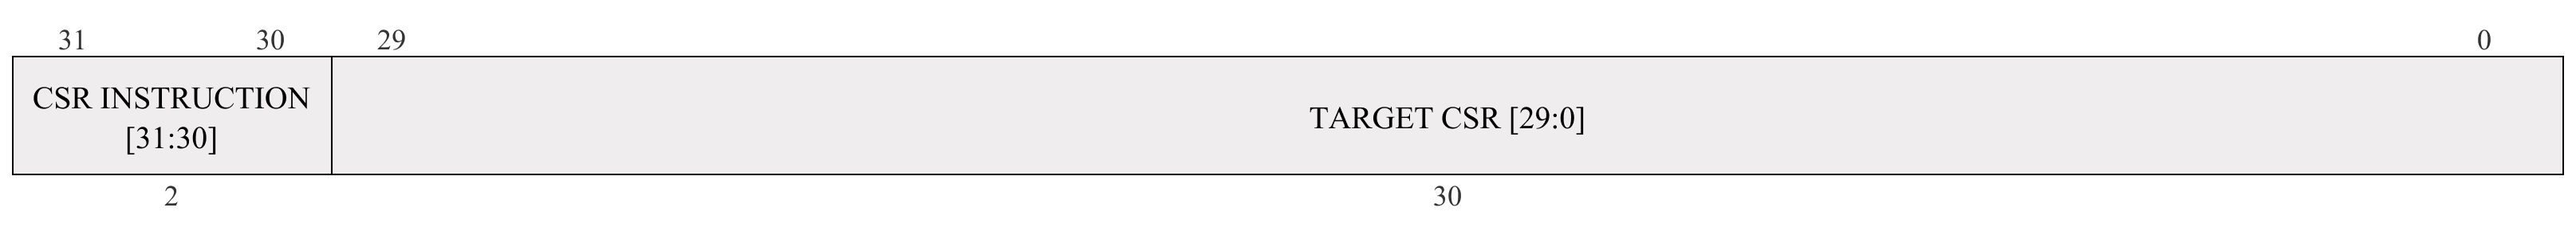
\includegraphics[width=.9\linewidth]{images/freertos_encoding.png}
  \caption{Possible encoding for register \textit{a6}}
  \label{fig:a6encoding}
\end{figure}\\

Inside the interrupt vector table, we would just need to add an if statement to determine
if we are requesting to perform a CSR instruction on behalf of \textit{FreeRTOS}
based on the \textit{ECALL} code.

Note that this is just a proposal of implementation and there are other ways to implement
\textit{FreeRTOS} inside \textit{STEERED}. For example, instead of encoding the CSR
instruction inside register \textit{a6}, we could define an \textit{ECALL} code
for each operation and simply use that value to determine the operation to
perform. This would result in fewer instructions to instrument (as we could
remove the \textit{or} instruction) but would increase the size of the handler
as we would need to provide controls for each implemented \textit{ecode}.
  \chapter{Future Works}
\label{cha:future}

In this thesis, we have seen that \textit{STEERED} poses itself as a
foundational approach to improving the security of \textit{RISC-V}-based embedded
systems. Moreover, it showed promising results in both the threat and performance
analysis, making it a suitable choice for real-world applications. However,
further advancements can enhance its applicability, efficiency, and robustness. This
chapter outlines potential directions for future work to expand the capabilities
of \textit{STEERED}. These future directions aim to establish \textit{STEERED}
as a cornerstone in the development of secure and efficient embedded systems. Addressing
these challenges will ensure its relevance and applicability in an ever-evolving
cybersecurity landscape.

\section{Additional Security Mechanisms}
\label{sec:future_security}

In previous chapters we discussed and demonstrated the ability of \textit{STEERED}
to detect and prevent control-flow attacks such as Return-Oriented Programming or
Jump-Oriented Programming. However, in security demanding environments it may be
necessary to introducer further techniques to protect the Control Flow Integrity
of the code. Here we list some security mechanisms that we plan to integrate in
\textit{STEERED}.

A \textit{Stack Canary} is a security mechanism used to detect and prevent stack-based
buffer overflow attacks, a common type of vulnerability in programs. It involves
placing a small, random value (the ``canary'') in memory just before the stack's
return address. This value acts as a sentinel and is checked for integrity
before the function returns control to its caller. If a buffer overflow occurs,
it overwrites memory beyond the intended bounds, which could potentially overwrite
the canary value before reaching the return address. Before the function returns,
the program compares the current canary value with the original value. If the
values differ, the program detects the overflow and terminates the execution to prevent
further exploitation. \textit{Stack Canaries} are simple yet effective as they provide
a straightforward way to detect stack corruption caused by buffer overflows,
also they are widely supported by many compilers. However, the process of
placing and checking canaries adds slight computational and memory overhead. Moreover,
\textit{Stack Canaries} only protect against stack-based buffer overflows,
leaving other memory regions vulnerable. In conclusion, we think that \textit{Stack
Canaries} would be a good addition to \textit{STEERED} as they would be easy to
implement and they provide a slight increase in security.

Since \textit{STEERED} suffers from source code modification as we have no way of
telling if the code was modified or not and this could affect the correctness of
forward and backward edge controls we could add an hashing function to the project.
With this function we could take the source code of \textit{STEERED} and generate
an hash. Note that we plan to take into account only the ``static'' part of
\textit{STEERED} and not the code imported by the user. With this we could
perform a check at each compilation by simply comparing the initial hash with
the freshly generated one. If the hash differs it means that the source code has
been tampered with and should not be trusted. This would lead to a simple and
fast way to determine if \textit{STEERED} is secure or if it has been modified.

Moreover, many device-specific security measures could be explored as there may
be some devices that provides hardware modules which could be used to further
increase the security of the project. However, this process requires exhaustive
testing and would lead to possible enhancement only on few embedded devices.

Note that we can't add security measures such as Data Execution Prevention (DEP)
or Address Space Layout Randomization (ASLR) to the binary as they would
conflict with \textit{STEERED}'s configuration. Data Execution Prevention
requires to set memory regions with either write but not execute privileges or
execute but not write privileges. This would obviously impact \textit{STEERED}
as it provides memory regions that requires both privileges. Address Space Layout
Randomization instead would randomize all the addresses so that they are different
at each execution. While this technique provides good security it would render
the Control Flow Graph completely useless as the addresses we collect during the
extraction would be different from the addresses at execution time leading to a
situation where each forward edge control fails.

Lastly, note that \textit{STEERED} is designed to protect the code from control-flow
attacks and must be paired with other security measures before deployment. This is
needed in order to ensure security on every attack surface. Otherwise, a threat actor
may be able to exploit other vulnerabilities to perpetrate an attack bypassing \textit{STEERED}'s
security features.

\section{Code Optimization}
\label{sec:future_optimization}

Although \textit{STEERED} has been designed with performance considerations, further
optimizations could enhance its usability in a broader range of embedded applications.
During the Performance Analysis in chapter \ref{cha:pa} we have seen that
\textit{STEERED} comes with an acceptable average time and space overhead.
However, there are edge cases where this is not true and the overhead grows exponentially.
In future works we plan to provide optimization solutions to cover such cases
lowering the time and space impact of \textit{STEERED} on the execution.

Firstly, we propose a solution to address the space overhead of deeply recursive
algorithms. We have seen that in these cases we need to allocate a very big Shadow
Stack which increases the size of the produced binary. To solve this, we propose
to add a \textit{peek} function which allows to look at the first element of the
Shadow Stack without removing it. When we need to perform a forward edge control
and consequently push the return address into the Shadow Stack we first check the
top value. If the addresses are the same we avoid pushing the same value more
times. On the other hand, when we need to perform a backward edge control we
look at the first value of the Shadow Stack. If the two addresses are equal we approve
the return instruction without popping the value. Instead, if the addresses differ,
we pop two values and compare the second one with the return address we are
checking. With this solution we could effectively address the problem with deeply
recursive algorithms without affecting the security capabilities of \textit{STEERED}.

Secondly, we provided a solution to reduce memory usage in cases where the user code
is small. For example, say that the user code starts at address $0x4038A000$ and
ends at address $0x4038F000$. Well, in this case we can ignore the first $16$ bits
of the address as they do not provide useful information. This means that we
could modify the Shadow Stack to store \textit{unsigned short} values instead of
\textit{unsigned int} values. Such a solution would halve the memory requirement
for the Shadow Stack. Although this solution is very effective in memory
management it is only applicable when the codebase is very small.

Moreover, we have seen that if the user-imported code is very big, take as an
example a firmware, the Control Flow Graph would drastically increase in size.
This is because, the larger the code, the larger is the possibility to have many
jump instruction from different source addresses to different destination
addresses. To address this problem, we propose to use an Hash Map instead of a
two dimensional array to represent the CFG. Although this solution does not reduce
memory usage, it allows for faster lookups as Hash Maps provide accesses in
constant time ($\mathcal{O}(1)$).

Lastly, converting the source code from \textit{C} language to pure \textit{Assembly}
language could increase performances and lead to further optimization solutions to
reduce time and memory overhead.

\section{Exhaustive Testing}
\label{sec:future_testing}

During the Threat Analysis in chapter \ref{cha:ta} we showcased the
effectiveness of \textit{STEERED} in protecting the Control Flow Integrity of the
user code. Moreover, we proved through tests that attempts to perform an unauthorized
control transfer are immediately detected and prevented by the Control Flow Integrity
Enforcer of \textit{STEERED}. However, we also pointed out that the presented
project is not able to mitigate non-control-flow attacks. In future works we plan
to perform exhaustive testing of the project to further inspect the behavior of \textit{STEERED}
in diverse environments. This could lead to either a stronger proof that \textit{STEERED}
is actually able to protect the code or to the discovery of untested scenarios. In
case of the latter we plan to provide a solution to eventual unexpected behavior.

\section{RTOS Implementation}
\label{sec:future_rtos}

The main focus for future works sees the integration of a Real-Time Operating
System such as \textit{FreeRTOS} or \textit{Zephyr RTOS} inside \textit{STEERED}.
Such task is of great importance due to the fact that an implementation
providing the features of both an RTOS and \textit{STEERED} would drastically increase
the number of fields in which this project could be used. In fact, this would open
door to more complex solution and would allow embedded devices to carry out complex
task within the secure execution environment provided by \textit{STEERED}.

  % Conclusions
  \chapter{Conclusions}
\label{cha:conclusions}

\lipsum[1]

  \endgroup

  % Bibliography
  \addcontentsline{toc}{chapter}{Bibliography}
  % Alphabetical order of authors
  \bibliographystyle{plain}
  \bibliography{bibliography.bib}

  % Attachments
  %\titleformat{\chapter} {\normalfont\Huge\bfseries}{Appendix \thechapter}{1em}{}
  %\appendix
  %\chapter{Attachment}
\label{cha:attachment}

\lipsum[1]
\end{document}
